

% --------------------------------------------------------------

% This is all preamble stuff that you don't have to worry about.

% Head down to where it says "Start here"

% --------------------------------------------------------------



\documentclass[titlepage]{report}
\PassOptionsToPackage{table,xcdraw,dvipsnames}{xcolor}

\usepackage[top=.75in,bottom=.75in,left=0.5in,right=0.5in]{geometry} 
\usepackage{amsmath,amsthm,amssymb,scrextend,mathtools,siunitx, cancel, bm, xfrac, esint}
\usepackage{mdframed}
\usepackage{csquotes}
\usepackage{tabto}
\usepackage{tikz}
\edef\restoreparindent{\parindent=\the\parindent\relax}
\usepackage{parskip}
\restoreparindent
\usepackage[hang,flushmargin,bottom]{footmisc}
\usepackage{longtable}
\usepackage{booktabs}

\usepackage{parskip,caption,gensymb}
\usepackage{graphicx,wrapfig,booktabs,multirow}
\usepackage{tabularx}
\usepackage{multicol}
\usepackage{placeins}
\usepackage{enumitem}
\graphicspath{./}
\usepackage{url}
\usepackage{fancyhdr,color,soul}
\usepackage{tikz}
\usepackage{textgreek}
\usepackage{float}
\usepackage{soul}
\usepackage{array}


\renewcommand{\baselinestretch}{1.5} %this is your line spacing, current at, you guessed it! 1.5
\pagestyle{fancy}
\setcounter{secnumdepth}{3}
\setcounter{tocdepth}{3}
\renewcommand{\thesection}{\arabic{section}}
\renewcommand{\thesubsection}{\thesection.\arabic{subsection}}
\renewcommand{\thesubsubsection}{\thesubsection.\arabic{subsubsection}}

\setcounter{secnumdepth}{3}
\setcounter{tocdepth}{3}


\usepackage[breaklinks=true,hidelinks]{hyperref} %remove [hidelinks] and all links will have box surrounding
\usepackage{changepage}
\usepackage{enotez}
\usepackage{bytefield}
\usepackage{tikz}
\usetikzlibrary{positioning}

\usepackage{xcolor}
\usepackage[fontsize=12pt]{fontsize}
\emergencystretch=2em
\setlist[itemize]{nosep,topsep=0pt,partopsep=0pt,parsep=0pt,itemsep=0pt}
\setlist[enumerate]{nosep,topsep=0pt,partopsep=0pt,parsep=0pt,itemsep=0pt}

\definecolor{codegreen}{rgb}{0,0.6,0}
\definecolor{codegray}{rgb}{0.5,0.5,0.5}
%\definecolor{lightgray}{rgb}{0.5,0.5,0.5}
\definecolor{codepurple}{rgb}{0.58,0,0.82}
\definecolor{backcolour}{rgb}{0.95,0.95,0.92}
\definecolor{backcolourt}{rgb}{0.95,0.95,0.92}
\definecolor{quotecolor}{rgb}{211,211,211}
\definecolor{chromeyellow}{rgb}{1.0, 0.65, 0.0}
\definecolor{Highlight}{HTML}{C04F17}
\definecolor{danger}{HTML}{800000}

\usepackage[draft,cache=false]{minted}
\usepackage[most,minted,breakable,skins]{tcolorbox}

\setminted[tasm]{%
	bgcolor=backcolour,
	linenos=true,
	breakanywhere=true,
	labelposition=topline,
	fontfamily=tt,
	fontsize=\footnotesize
}
\usemintedstyle{xcode}

\newtcblisting[number format=\arabic]{code}[2]
{
	listing engine=minted,
	minted language=#1,
	minted options={mathescape, breaklines=true, breakanywhere=true, fontfamily=tt, fontsize=\footnotesize},
	listing only,
	breakable,
	enhanced,
	colback=backcolour!10,
	coltitle=white,  
	title={#2},
}

\tcbset{breakable}

% if you want to define a new color use this format: {name}{RBG}{R, G, B values}
%\definecolor{teal}{RGB}{0, 128, 128 } 
\definecolor{ltgray}{gray}{0.95}

\renewcommand{\thefootnote}{\arabic{footnote}}

\newcommand*{\hamil}{\hat{\mathcal{H}}}


\newcommand{\N}{\mathbb{N}}

\newcommand{\Z}{\mathbb{Z}}

\newcommand{\I}{\mathbb{I}}

\newcommand{\R}{\mathbb{R}}

\newcommand{\Q}{\mathbb{Q}}

\renewcommand{\qed}{}

\let\newproof\proof



\renewenvironment{proof}{\begin{mdframed}[backgroundcolor=ltgray]\begin{addmargin}[1mm]{1mm}\footnotesize\begin{newproof}}{\end{newproof}\end{addmargin}\end{mdframed}\qed}
% \newcommand{\expl}[1]{\text{\hfill[#1]}$}

\newenvironment{theorem}[2][Theorem]{\begin{trivlist}
		
		\item[\hskip \labelsep {\bfseries #1}\hskip \labelsep {\bfseries #2.}]}{\end{trivlist}}


\newenvironment{lemma}[2][Lemma]{\begin{trivlist}
		
		\item[\hskip \labelsep {\bfseries #1}\hskip \labelsep {\bfseries #2.}]}{\end{trivlist}}

\newenvironment{problem}[2][Problem]{\begin{trivlist}
		
		\item[\hskip \labelsep {\bfseries #1}\hskip \labelsep {\bfseries #2.}]}{\end{trivlist}}

\newenvironment{exercise}[2][Exercise]{\begin{trivlist}
		
		\item[\hskip \labelsep {\bfseries #1}\hskip \labelsep {\bfseries #2.}]}{\end{trivlist}}

\newenvironment{reflection}[2][Reflection]{\begin{trivlist}
		
		\item[\hskip \labelsep {\bfseries #1}\hskip \labelsep {\bfseries #2.}]}{\end{trivlist}}

\newenvironment{proposition}[2][Proposition]{\begin{trivlist}
		
		\item[\hskip \labelsep {\bfseries #1}\hskip \labelsep {\bfseries #2.}]}{\end{trivlist}}

\newenvironment{corollary}[2][Corollary]{\begin{trivlist}
		
		\item[\hskip \labelsep {\bfseries #1}\hskip \labelsep {\bfseries #2.}]}{\end{trivlist}}

\setminted{
	breaklines=true,
	breakanywhere=true
}

\newtcolorbox{functionspec}[1]{%
	breakable,
	enhanced,
	borderline north = {.5mm}{0mm}{blue},
	arc=0pt,
	outer arc=0pt,
	colframe=white,
	colback=white,
	coltitle=blue!70!black,
	fonttitle=\ttfamily\normalsize\bfseries,
	fontupper=\ttfamily,
	boxed title style={empty},
	title={#1}}

\usepackage{setspace}
\newtcolorbox{notespec}{
	breakable,
	enhanced,
	frame empty,
	borderline west = {1.5mm}{0mm}{yellow},
	fontlower=\bfseries,
	fontupper=\bfseries,
	colback=white,
	colback=yellow!5
}

\newtcolorbox{warningspec}{
	breakable,
	enhanced,
	frame empty,
	borderline west = {1.5mm}{0mm}{red},
	fontlower=\bfseries,
	fontupper=\bfseries,
	colback=white,
	colback=red!5
}

\newtcolorbox{newquote}{
 breakable,
enhanced,
frame empty,
leftrule=1.5pt,
rightrule=0pt,
toprule=0pt,
bottomrule=0pt,
borderline west={1.5pt}{0pt}{black!60},
colback=gray!5,
fontupper=\footnotesize
}
\setlength{\parindent}{0pt}

\newcommand{\critical}[1]{{\color{danger}\textbf{#1}}}
\newcolumntype{C}{>{\centering\arraybackslash}p{1.6cm}}
\renewcommand{\arraystretch}{1.5}

% --------------------------------------------------------------

%                         Start here

% --------------------------------------------------------------



%\lhead{left}

%\chead{center}

%\rhead{Right}

%If you uncomment any/all of the above, you can set your own headers, uncommenting one will remove the auto headers in place (section and subsection) 


\makeatletter\@enumdepth1\makeatother

\makeatletter
\def\@Aboxed#1&#2&#3\ENDDNE{%
	\ifnum0=`{}\fi \setbox \z@
	\hbox{$\displaystyle#1{}\m@th$\kern\fboxsep \kern\fboxrule }%
	\edef\@tempa {\kern  \wd\z@ &\kern -\the\wd\z@ \fboxsep
		\the\fboxsep \fboxrule \the\fboxrule }\@tempa 
	\fcolorbox{white}{ltgray}{$\displaystyle #1#2$}% changed
}
\makeatother
\begin{document}
	
	\begin{titlepage}
		\begin{center}
			\vspace*{1in}
			{\Large\textbf{lwIP-CE with TLS 1.3\\Whitepaper}}\\
			\vspace*{0.5in}
			{\huge\textbf{Analysis\\\vspace{10px}Justifications}}\\
			\vspace*{1in}
			by Anthony Cagliano
		\end{center}
	\end{titlepage}
	\setcounter{secnumdepth}{2}
	\setcounter{tocdepth}{2}
	\tableofcontents	
	
	\newpage
	\section{Foreword}
	The \textbf{lwIP-CE} project is an adaptation and integration of the Lightweight IP (lwIP) stack for highly constrained embedded systems, specifically targeting the TI-84+ CE platform and similar resource-limited environments. This work represents a deliberate effort to bring modern networking capabilities—including Ethernet, IPv4/IPv6, and TLS—to hardware never originally designed for full internet participation.
	
	Traditional networking stacks assume megabytes of memory, preemptive multitasking, and operating systems with dynamic resource management. The TI-84+ CE provides none of these conveniences. Instead, it offers a single-threaded execution model, limited RAM, no native networking abstraction, and tight timing constraints on a 48 MHz processor. Yet despite these constraints, the goal of lwIP-CE is not merely “minimal networking,” but correct, standards-aligned, interoperable networking.
	
	This whitepaper documents the architecture, design decisions, trade-offs, and implementation details behind lwIP-CE. It covers the layering model from USB driver integration through Ethernet abstraction and into the lwIP stack, as well as the TLS implementation constraints and cryptographic considerations required on this class of device.
	
	lwIP-CE is not intended to turn a calculator into a server farm. It is predominately a proof of concept and capability, an engineering exploration, and a platform for experimentation in secure embedded networking. It demonstrates that: 
	\begin{itemize}
	\item Modern TCP/IP stacks can be responsibly adapted to deeply constrained systems.
	\item TLS with contemporary cipher suites is feasible within tight memory and performance limits.
	\item Clean architectural boundaries (USB,  Ethernet, lwIP, TLS) allow portability and long-term maintainability even in non-traditional environments.
	\end{itemize}
	
	This document is intended for:
	\begin{itemize}
	\item Embedded systems developers
	\item Networking and protocol engineers
	\item Security researchers
	\item Contributors evaluating or auditing the design
	\item Advanced calculator developers exploring networked applications
	\end{itemize}
	
	The reader is assumed to have familiarity with TCP/IP fundamentals, embedded systems design, and basic cryptographic concepts.
	
	I am fully aware that many readers, particularly within the cryptography community, will invoke the well-known principle: "Don't roll your own crypto". On platforms where mature, audited cryptographic libraries exist, that principle is not only sound but essential. The TI-84+ CE, however, offers no such luxury. When I began work on CryptX several years ago, it was a proof of concept and a personal learning exercise. Over time, it evolved beyond experimentation. The calculator community responded positively, and I discovered that I genuinely valued both the engineering challenge and the responsibility that came with it.
	
	When the scope expanded from standalone cryptographic primitives to a full TLS 1.3 implementation integrated with lwIP, the standards changed. The margin for error narrowed. The expectations rose. This document reflects that shift. Every design decision, optimization, constraint, and trade-off was examined with care. While no implementation on a platform this heavily constrained can claim perfection, this work represents a deliberate, disciplined effort to pursue correctness, interoperability, and security to the fullest extent the hardware permits.
	
	This project -- along with the associated research, sustained study and research -- is where I learned most of what I now know about cryptography. In that sense, it achieved its core purpose. Even where the implementation is imperfect, the technical growth has been substantial. Early iterations reflected the exploratory nature of the work; over time, the project matured alongside a deeper understanding of cryptographic rigor. I include that candidly, not as self-criticism, but as context for how much this work changed my engineering standards. At the time of writing, I have a materially stronger grasp of the field, including why “good enough” is not adequate for security work, how to design around logical, mathematical, and statistical rigor, and how to document and own security-relevant tradeoffs explicitly.
	
	\newpage
	\section{Stack Adaptations and Extensions}
	\label{sec:implementation_overview}
	
		Before examining the architecture and technical details, an important disclaimer is necessary.
		
		This implementation is designed to be RFC-compliant and is informed by FIPS-aligned design principles; however, it is not FIPS-certified, nor has it undergone formal third-party cryptographic audit beyond review within the TI-84+ CE development community. Any security assurances provided by this project should therefore be considered provisional and contextual.
		
		These limitations are not the result of neglect, but of constraint. The TI-84+ CE platform imposes strict trade-offs between computational performance, memory usage, and defensive hardening. Certain implementation decisions reflect careful balancing between theoretical ideal and practical feasibility on a 48 MHz, resource-limited system.
		
		That said, this document is written with full transparency. The architecture, cryptographic constructions, mitigation, and design rationale are laid out in detail. Readers are encouraged to evaluate the implementation on its merits. You may find that the conservatism expressed here exceeds what the engineering decisions ultimately warrant.
		
		\subsection{Adapting lwIP to the TI-84+ CE}
		The initial porting effort was undertaken by Cemetech user \textit{commandblockguy}, who prepared lwIP for the TI-84+ CE environment by isolating and conditionally excluding features incompatible with the calculator’s execution model. This included removing OS-dependent functionality, threading assumptions, and unsupported memory abstractions, while preserving protocol correctness.
		
		A more substantial challenge arose from the calculator’s atypical integer model. The eZ80 CPU operates in a 24-bit address and data environment, and under the CE toolchain, the fundamental C types differ from conventional 32-bit architectures. In particular:
		\begin{itemize}
		\item \texttt{short} is 16 bits
		\item \texttt{int} is 24 bits
		\item \texttt{long} is 32 bits (implemented as multi-register operations)
		\end{itemize}
		At the time of the original port, support for integer widths beyond 32 bits was limited, requiring careful handling of any operations that assumed native 32-bit promotion semantics. Arithmetic exceeding 24 bits incurs compiler-generated multi-register sequences, and operations beyond 32 bits required explicit multiprecision handling.
		
		Subsequent revisions of the toolchain introduced additional fixed-width types (e.g., 48-bit and 64-bit integers), allowing portions of earlier compatibility workarounds to be simplified or reverted. Nevertheless, all lwIP fixed-width types were explicitly audited to ensure that their effective widths and promotion behavior matched protocol expectations.
		
		
\subsection{Stack Architecture Overview}

Before beginning this project we needed to itemize what was available and what was needed. The chart below shows the TCP/IP and OSI layer, and what components are assigned to that layer.

\begin{table}[h]
	\centering
	\begin{tabularx}{\textwidth}{C C l X}
		\toprule
		\textbf{TCP/IP Layer} & \textbf{OSI Layer} & \textbf{Component} & \textbf{Function} \\
		\midrule
		
		1 $\leftrightarrow$ 2 & 1--2 & USBDRVCE &
		Hardware transport interface for USB host communication. Handles device
		enumeration, endpoint transfers, and interrupt-driven USB activity used
		by Ethernet adapters. \\
		
		2 & 2 & CDC ECM / NCM Ethernet &
		Ethernet data link layer provided by USB CDC-class adapters. Responsible
		for Ethernet frame encapsulation, MAC addressing, and link state
		notifications. \\
		
		3 $\leftrightarrow$ 4 & 3--4 & lwIP &
		Core networking stack implementing IP, ARP, ICMP, IPv6, TCP, and UDP.
		Provides packet routing, protocol handling, and socket-style networking
		interfaces. \\
		
		5 & 5--7 & ALTCP, TLS, Application &
		High-level abstractions exposed to calculator programs. ALTCP provides a
		transport wrapper allowing optional TLS integration, while TLS provides
		confidentiality, integrity, and endpoint authentication for application
		data. \\
		
		\bottomrule
		
	\end{tabularx}
	
	\caption{Relationship between the lwIP-CE networking architecture, the TCP/IP model, and the OSI model.}
\end{table}
		
		
		\subsection{USB CDC-Class Ethernet driver}
		To provide reliable networking on TI-84+ CE hardware, a USB CDC Ethernet host driver was implemented for ECM (Ethernet Control Model) and NCM (Network Control Model) adapters. These are the common CDC Ethernet profiles available on commodity USB dongles and provide the broadest practical compatibility.

		The implementation is layered on \texttt{USBDRVCE} (toolchain USB library by jacobly). \texttt{USBDRVCE} owns low-level bus/device lifecycle handling; the CDC layer focuses on class parsing, endpoint wiring, and forwarding frames into lwIP.

		Initialization starts from the USB callback path and performs descriptor parsing for hubs and CDC-capable devices. The metadata extracted includes:
		\begin{itemize}
			\item The configuration/interface containing the CDC ECM/NCM subclass (vendor-specific configurations often appear first).
			\item Bulk RX, bulk TX, and interrupt endpoint descriptors.
			\item MAC address via descriptor string, or fallback control request.
			\item For NCM, the NCM functional descriptor and NTB capability fields.
		\end{itemize}

		After discovery, the driver applies CDC setup:
		\begin{enumerate}
			\item \texttt{SetConfiguration} to the CDC-capable configuration.
			\item \texttt{SetInterface} to the selected bulk transfer interface.
			\item If MAC retrieval fails, generate a valid local MAC and program it via control request.
			\item For NCM we perform the following additional actions:
				\begin{enumerate}
					\item Query NTB parameters.
					\item Set NTB input size to a small supported size (typically 2048 bytes) to keep RX bursts manageable on CE.
					\item Apply packet filter/multicast controls when supported.
				\end{enumerate}
			\item Bind RX/TX/interrupt callbacks into \texttt{eth\_device\_t} and attach the lwIP \texttt{netif}.
		\end{enumerate}

		Interrupt-endpoint handling is intentionally narrow. For CDC ECM/NCM on this platform, only one notification is operationally relevant:
		\begin{itemize}
			\item \textbf{NetworkConnection}: maps directly to \texttt{netif} link up/down state through \texttt{wValue}.
		\end{itemize}
		Other CDC notifications (for example \texttt{NetworkSpeedChange}) are either non-actionable for this target or already covered at lower driver layers.

		RX ingress is decoupled from callback latency via scheduled bulk reads and a ring-buffer drain timer, so frame ingestion remains bounded under memory pressure.

		Operational workflow, condensed:
		\begin{enumerate}
			\item USB connect/enable events trigger CDC descriptor discovery and configuration.
			\item Endpoints and MAC identity are resolved; ECM or NCM callbacks are bound.
			\item Interrupt callback tracks \texttt{NetworkConnection} and updates link status.
			\item RX scheduling/draining timers move bulk data into lwIP while honoring memory-throttle policy.
			\item Disconnect/disable transitions force link-down and cleanup/reset of endpoint state.
		\end{enumerate}
		
		The driver also defines a fatal-error state entered on non-recoverable endpoint stall. In that state, the device is reset, which:
		\begin{itemize}
			\item unschedules callbacks bound to the affected device;
			\item clears endpoint halt/stall and related transfer error state; and
			\item triggers a subsequent \texttt{ENABLED} event, restarting the normal device-initialization sequence.
		\end{itemize}
		
		This driver provides robust, platform-appropriate USB Ethernet transport for lwIP on TI-84+ CE hardware. By constraining scope to CDC ECM/NCM, prioritizing deterministic recovery on endpoint failure, and decoupling RX ingestion through scheduled drain/throttle control, the implementation achieves stable link behavior under low memory and timing constraints.
		
	
		\subsection{Membuffer "driver"}
		In addition to the USB driver, a dedicated \texttt{membuffer} allocator layer was implemented to keep memory behavior predictable across lwIP, USB RX/TX staging, and TLS components. On this platform, allocator stability is a correctness property: when memory pressure spikes, transport behavior and security-sensitive state handling must degrade in a controlled way rather than fail unpredictably.

		The subsystem supports two initialization modes:
		\begin{itemize}
		 \item \textbf{Dynamic mode}: wraps toolchain \texttt{malloc}/\texttt{free}/\texttt{realloc} with explicit heap accounting and pressure reporting.
		\item \textbf{Static mode}: uses a caller-provided arena with fixed bounds and no external allocator dependency after initialization.
		\end{itemize}

		Within either mode, \texttt{membuffer} provides three buffer classes tuned to workload shape:
		\begin{itemize}
			\item \texttt{MEM\_BUFFER\_RING}: FIFO streaming buffers (used by asynchronous ingress paths such as USB RX).
			\item \texttt{MEM\_BUFFER\_POOL}: block-style allocations for frequent alloc/free traffic.
			\item \texttt{MEM\_BUFFER\_FILE}: slot-based, lazy file I/O allocation.
		\end{itemize}

		The dynamic path includes pressure-aware sizing controls (grow/shrink thresholds, step sizing, hold logic, and per-buffer max caps) plus pressure callbacks. Pressure levels are tiered (\texttt{NONE} $\rightarrow$ \texttt{MILD} $\rightarrow$ \texttt{HIGH} $\rightarrow$ \texttt{SEVERE} $\rightarrow$ \texttt{CRITICAL}), with optional global pressure signaling to coordinate cross-module throttling.

		This is directly coupled to the Ethernet ingress path: RX ring buffers use drain callbacks and timer-driven budgets, while pressure callbacks adjust scheduling/throttle behavior under load. In practice, this allows the stack to keep link handling responsive while avoiding runaway allocation during bursts.

			From a security perspective, buffers can be flagged with \texttt{BUFFER\_SECURE\_MODE}, enabling automatic zeroization on pop/free/release paths. This does not replace higher-layer cryptographic hygiene, but it materially reduces residual plaintext/key exposure in normal allocator lifecycles.

			\subsection{Operational Memory Characteristics}

			The lwIP-CE stack's memory footprint is composed of fixed-size BSS structures (memp pools, USB driver state) and dynamically-sized buffers that grow with traffic and connection count. The \textit{Idle} column shows what is allocated at rest --- the default sizes of all buffers and pools that exist persistently regardless of activity. The \textit{Peak} column shows the largest each component grows to under load. All figures assume the eZ80 ABI (3-byte pointers) and the default sizing constants in \texttt{lwipopts.h}; constants in parentheses are the configuration knobs that govern each row.

			\refstepcounter{table}\label{tab:lwip-memory}
			\textbf{Table \thetable: Memory footprint of the full lwIP-CE stack, grouped by allocation lifetime.}

			\begingroup
			\setlength{\tabcolsep}{3pt}
			\setlength{\LTleft}{0pt}
			\setlength{\LTright}{0pt}
				\begin{longtable}{>{\raggedright\arraybackslash}p{0.24\textwidth}p{0.10\textwidth}p{0.18\textwidth}p{0.38\textwidth}}
					\toprule
					\textbf{Component} & \textbf{Idle} & \textbf{Peak} & \textbf{Notes} \\
					\midrule
				\endfirsthead
					\toprule
					\textbf{Component} & \textbf{Idle} & \textbf{Peak} & \textbf{Notes} \\
					\midrule
				\endhead
					\bottomrule
				\endfoot
						\multicolumn{4}{p{0.90\textwidth}}{\textit{Fixed state structures --- always allocated, never grow}} \\
					\midrule
					TCP PCB pool                   & ${\sim}3{,}520$ & ${\sim}3{,}520$ & \texttt{MEMP\_NUM\_TCP\_PCB} (16) $\times$ ${\sim}220\,\text{B}$ \\
					TCP segment pool               & ${\sim}960$ & ${\sim}960$ & \texttt{MEMP\_NUM\_TCP\_SEG} (32) $\times$ ${\sim}30\,\text{B}$ \\
					TCP listen-PCB pool            & ${\sim}280$ & ${\sim}280$ & \texttt{MEMP\_NUM\_TCP\_PCB\_LISTEN} (4) $\times$ ${\sim}70\,\text{B}$ \\
					ALTCP PCB pool                 & ${\sim}560$ & ${\sim}560$ & \texttt{MEMP\_NUM\_ALTCP\_PCB} (16) $\times$ ${\sim}35\,\text{B}$ \\
					UDP PCB pool                   & ${\sim}220$ & ${\sim}220$ & \texttt{MEMP\_NUM\_UDP\_PCB} (4) $\times$ ${\sim}55\,\text{B}$ \\
					sys\_timeout pool              & ${\sim}384$ & ${\sim}384$ & \texttt{MEMP\_NUM\_SYS\_TIMEOUT} (32) $\times$ ${\sim}12\,\text{B}$ \\
					ARP table                      & ${\sim}300$ & ${\sim}300$ & \texttt{ARP\_TABLE\_SIZE} (10) \\
					USB-Ethernet driver state      & ${\sim}2{,}200$ & ${\sim}2{,}200$ & MAC config, descriptor scratch, NCM buffers \\
					DRBG / RNG state               & ${\sim}80$ & ${\sim}80$ & DRBG context + RNG queue heads \\
					\midrule
						\multicolumn{4}{p{0.90\textwidth}}{\textit{Pools and buffers with idle minimums --- grow on demand, shrink back}} \\
					\midrule
					USB-Ethernet RX ring           & $512$ & $2{,}048$ & \texttt{ETH\_RX\_RING\_\{INIT,MAX\}\_SIZE} \\
					Pbuf pool (demand-driven)      & ${\sim}0$ & up to cap & Allocated through custom allocator (\texttt{MEMP\_MEM\_MALLOC}); pays for in-flight TCP data, including encrypted TLS records retained until processed \\
					lwIP MEM heap (demand-driven)  & ${\sim}0$ & up to cap & Backs outbound TCP segments, retransmit queue, transient lwIP scratch \\
					\midrule
						\multicolumn{4}{p{0.90\textwidth}}{\textit{TLS-specific --- only allocated when the TLS stack is in use}} \\
					\midrule
					TLS handshake context          & ${\sim}880$ & ${\sim}880$ & Per connection; lifetime = TLS connection \\
					altcp\_tls\_ce state           & ${\sim}150$ & ${\sim}150$ & Per connection; lifetime = TLS connection; owns queued encrypted pbuf chain \\
					Decrypted TLS record scratch   & $0$ & ${\sim}16{,}384$ & Per connection; transient; used only after a complete encrypted record is present \\
					Handshake reassembly buffer    & $0$ & up to ${\sim}4{,}096$ & Per connection; transient; allocated only for non-Certificate handshake messages fragmented across TLS records (\texttt{EncryptedExtensions}, \texttt{Finished}, \texttt{NewSessionTicket}) \\
					Certificate streaming walker   & $0$ & ${\sim}1{,}024$--$5{,}120$ & Per connection; transient; one cert's DER allocated at a time, freed after SPKI check; replaces full-chain buffering for \texttt{Certificate} messages \\
					RSA padding pool               & $0$ & $1{,}024$ & Shared across all TLS connections; lazy, allocated on first RSA op \\
					\midrule
					\textbf{Stack baseline (no TLS conn)}  & \textbf{${\sim}9\,\text{KiB}$}  & \textbf{${\sim}10.5\,\text{KiB}$} & Fixed structures + USB ring at peak \\
					\textbf{Per-TLS-conn delta}            & \textbf{${\sim}1\,\text{KiB}$}  & \textbf{${\sim}18\,\text{KiB}$} typical / \textbf{${\sim}23\,\text{KiB}$} fragmented & TLS section, per active connection, excluding encrypted pbuf payloads \\
					\textbf{Total (1 TLS conn active)}     & \textbf{${\sim}11\,\text{KiB}$} & \textbf{${\sim}29\,\text{KiB}$} typical / \textbf{${\sim}34\,\text{KiB}$} fragmented & Plus whatever the demand-driven pools claim from the cap \\
			\end{longtable}
			\endgroup

			TLS receive processing is intentionally pbuf-backed. Encrypted TCP input is kept as an ordered pbuf chain owned by the connection; the stack waits until a complete TLS record is available, then decrypts that record directly from the pbuf chain. Application-data records decrypt into the final plaintext pbuf handed upward, while handshake records decrypt into one transient plaintext buffer so the existing handshake parser and cross-record reassembly logic can remain centralized. The encrypted pbuf bytes are freed and acknowledged to TCP only after the record has been authenticated and processed.

			A single-TLS-connection deployment now peaks at roughly $29\,\text{KiB}$ for a typical single-record handshake Certificate path --- the $10.5\,\text{KiB}$ baseline plus about $1\,\text{KiB}$ of per-connection TLS state, one decrypted record scratch buffer, and the shared RSA padding pool. A deliberately fragmented Certificate message raises this toward $34\,\text{KiB}$, because the decrypted record scratch and the per-cert walker buffer may coexist briefly; the walker allocates at most one cert's DER at a time ($1$--$5\,\text{KiB}$ typical) and frees it immediately after the SPKI check, so the old full-chain buffering peak of ${\sim}16\,\text{KiB}$ is eliminated. Non-Certificate handshake messages that span TLS records still use flat reassembly, but those messages are small (at most a few KiB for \texttt{NewSessionTicket}), keeping fragmented overhead well below the former ceiling. Demand-driven lwIP work (outbound TCP segments, queued encrypted pbufs) adds whatever the application's workload calls for, bounded by the global allocator cap. For multi-connection deployments, add roughly $1\,\text{KiB}$ per additional idle TLS connection and budget the transient decrypted-record/reassembly cost per concurrent handshake.

			Memory pressure is observed by the global \texttt{membuffer} accountant. Under \texttt{MILD} or \texttt{HIGH} pressure, propagation of \texttt{altcp\_recved} to TCP is divided down, slowing wire-side ingestion; under \texttt{CRITICAL} pressure it is suppressed entirely. New TLS connections opened during pressure thus run, but degrade in throughput rather than fail outright.

			\subsubsection{User-Tunable Memory Budget}

			On the TI-84+ CE the application shares roughly $60\,\text{KiB}$ of working RAM with the network stack, so the per-buffer defaults above leave little headroom for the host application. Rather than expose a fistful of per-buffer ceilings, the configurator exposes a single knob: \texttt{lwip\_mem\_cap}, the total number of bytes given to the lwIP global allocator. At boot this value is passed directly to \texttt{mem\_init}:
			\[
				\texttt{mem\_init}(\texttt{lwip\_mem\_cap}, \ldots)
			\]
			All lwIP-side allocations --- pbufs, MEM heap, TLS scratch buffers, USB driver buffers --- charge against this single budget. The RAM above the cap remains untouched by lwIP, available to the host application:
			\[
				\text{usermem\_remaining} = \text{free\_ram} - \texttt{lwip\_mem\_cap}
			\]

			The configurator presents an interactive breakdown while the knob is being adjusted:
			\begin{itemize}
				\item \textbf{Fixed structures} --- the always-resident pool and state overhead (${\sim}9\,\text{KiB}$ baseline).
				\item \textbf{TLS (if active)} --- the minimum working set for one TLS connection (${\sim}15\,\text{KiB}$, only shown when TLS is enabled).
				\item \textbf{Remaining pbuf pool} --- cap minus the above fixed overhead; this is the headroom available for dynamic pbuf and heap growth.
				\item \textbf{Usermem remaining} --- free RAM above the cap, left for the host application.
			\end{itemize}

			The configurator enforces a minimum: \texttt{lwip\_mem\_cap} cannot be set below \texttt{LWIP\_MIN\_FLOOR\_BYTES} ($24\,\text{KiB}$ when TLS is enabled, $12\,\text{KiB}$ otherwise). This floor reflects the minimum working set required for one ordinary TLS connection through handshake. A stored configuration that exceeds current free RAM (e.g.\ because the user installed more apps since last save) is clamped down at boot before \texttt{mem\_init} is called.

			This design trades the precision of per-buffer ceilings for a single, intuitive knob whose semantics match what the stack actually receives. Buffers grow into the available cap as traffic demands and shrink back when it quiets, so an idle TLS session leaves nearly all of the cap available for other lwIP work; only during peak load (a Certificate message, a burst of records) does lwIP approach its allocator ceiling.

			\subsection{Application Callability}
			lwIP-CE is intended to operate as a resident networking component that other calculator programs can call, rather than as a program whose networking stack is statically copied into each consumer. I was intent on making this library callable in place rather than statically included because the lwIP core and TLS internals are huge (around 200KB) and on a device with just under 2MB of Flash storage, this adds up quickly. This design reduces duplicated code size, centralizes network state, and allows application programs to depend on a stable exported interface.
			
			The calculator environment does not provide conventional shared-library loading in the desktop sense. The TI-84+ CE toolchain provides a dispatch utility for loading on-device libraries called \texttt{LIBLOAD}. This utility normally works through:
			\begin{itemize}
				\item A series of C- or assembly-callable functions that perform some action and return.
				\item An exports table listing every function that should be part of the public API.
				\item \textbf{During linking}: exports are converted into a jump table, in export order, where each jump target is represented as an offset to the exported function.
				\item \textbf{At program initialization}: a LibLoad bootstrap function locates the library in memory and combines the library base address with the stored offsets to produce callable entry points.
				\item \textbf{At API call}: \verb|call my_api| targets a stub entry that dispatches to the resolved implementation address.
			\end{itemize}


			The issue here is that this model targets small AppVar libraries that can live in RAM for their usage cycle and is not designed to support Applications as the API source. This requires a slightly different engineering solution.

			\begin{itemize}
				\item A table of exports is linked into the application, similarly to how \texttt{LIBLOAD} handles library exports.
				\item The export table must either live at a consistent location across builds or have its location recorded in an unused application-header field.
				\item A small \texttt{LIBLOAD} companion library provides consumer-side stubs and a bootstrap function. The bootstrap locates the installed lwIP application, resolves the application export table, and patches or populates the local stubs so later API calls dispatch into the resident application.
			\end{itemize}

			Concretely, the implementation realizes this with three cooperating pieces. The lwIP application links an \emph{export table} into its own image: a six-byte magic marker (\texttt{"LWIPTB"}) followed by one entry per public symbol, each stored as that symbol's offset from the application base. Because applications link at a base of zero, an entry's link-time address \emph{is} its offset, so no base subtraction is needed at generation time. The table's position is not guessed at runtime; a build step records the byte offset to it (\texttt{\_\_lwip\_fn\_table\_off}) and bakes that constant into the companion library. The \emph{companion library} is an ordinary \texttt{LIBLOAD} library the consumer links against; it carries one jump-table trampoline per exported lwIP function plus an imports table (host CRT slots and the USB vtable). At runtime, a \emph{bootstrap} routine ties the two together.

			\subsubsection{Initialization Handshake}
			Bringing the stack up happens in two stages: the ordinary \texttt{LIBLOAD} initialization of the companion library, followed by lwIP-CE's own runtime setup, triggered explicitly when the consumer calls \texttt{lwip\_init\_runtime(malloc, free, realloc)}. Figure~\ref{fig:libload_bootstrap} traces the full sequence. The key ordering constraint is that the application's own initialization (\texttt{lwip\_init\_runtime\_internal}) is itself an exported call, so it can only run \emph{after} the trampolines have been patched --- the bootstrap reaches into the app to finish setting up the app.

			\begin{figure}[H]
				\centering
				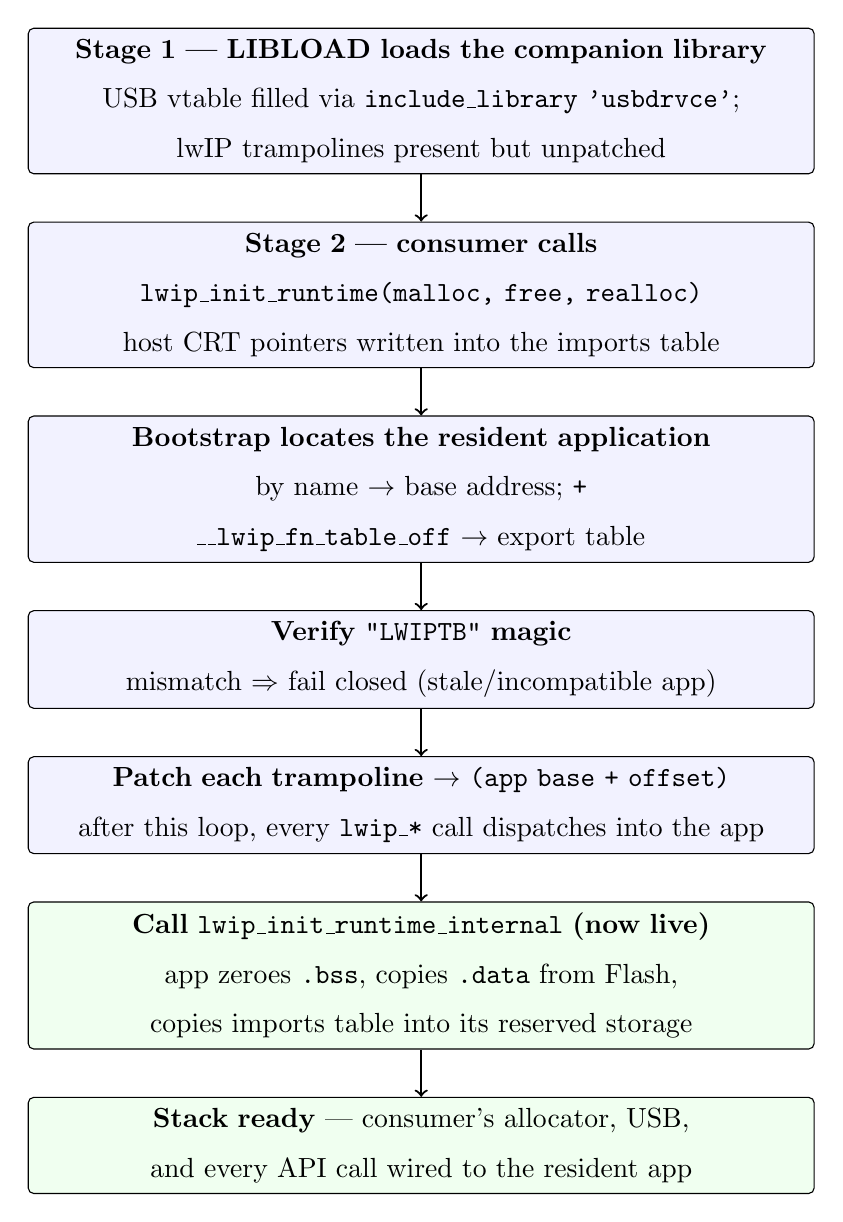
\begin{tikzpicture}[
					font=\footnotesize,
					node distance=6mm,
					box/.style={draw, rounded corners=2pt, align=center,
						text width=0.80\textwidth, inner sep=4pt},
					lib/.style={box, fill=blue!5},
					app/.style={box, fill=green!6},
					flow/.style={->, thick}
				]
					\node[lib] (load) {\textbf{Stage 1 --- LIBLOAD loads the companion library}\\
						USB vtable filled via \texttt{include\_library 'usbdrvce'}; lwIP trampolines present but unpatched};
					\node[lib, below=of load] (call) {\textbf{Stage 2 --- consumer calls} \texttt{lwip\_init\_runtime(malloc, free, realloc)}\\
						host CRT pointers written into the imports table};
					\node[lib, below=of call] (find) {\textbf{Bootstrap locates the resident application}\\
						by name $\rightarrow$ base address; \texttt{+ \_\_lwip\_fn\_table\_off} $\rightarrow$ export table};
					\node[lib, below=of find] (verify) {\textbf{Verify} \texttt{"LWIPTB"} \textbf{magic}\\
						mismatch $\Rightarrow$ fail closed (stale/incompatible app)};
					\node[lib, below=of verify] (patch) {\textbf{Patch each trampoline} $\rightarrow$ \texttt{(app base + offset)}\\
						after this loop, every \texttt{lwip\_*} call dispatches into the app};
					\node[app, below=of patch] (internal) {\textbf{Call} \texttt{lwip\_init\_runtime\_internal} \textbf{(now live)}\\
						app zeroes \texttt{.bss}, copies \texttt{.data} from Flash, copies imports table into its reserved storage};
					\node[app, below=of internal] (ready) {\textbf{Stack ready} --- consumer's allocator, USB, and every API call wired to the resident app};

					\draw[flow] (load) -- (call);
					\draw[flow] (call) -- (find);
					\draw[flow] (find) -- (verify);
					\draw[flow] (verify) -- (patch);
					\draw[flow] (patch) -- (internal);
					\draw[flow] (internal) -- (ready);
				\end{tikzpicture}
				\caption{\footnotesize LIBLOAD dispatch and bootstrap flow. Stage~1 is ordinary \texttt{LIBLOAD} library init (blue); Stage~2 is lwIP-CE's custom runtime setup, triggered by \texttt{lwip\_init\_runtime}, ending with the app's own initialization (green). The three host C-runtime pointers are stored before the app is located; the app's \texttt{.bss}/\texttt{.data} init and imports-table copy run last, through the now-patched table.}
				\label{fig:libload_bootstrap}
			\end{figure}

			\subsubsection{Runtime Memory Contract}
			Because the application's \texttt{.bss} and \texttt{.data} are initialized at runtime rather than at launch, they require a fixed RAM home that does not collide with the consumer program's own variables. lwIP-CE reserves a 6\,KiB window from the toolchain's default \texttt{BSSHEAP\_LOW} (\texttt{0xD052C6}) up to \texttt{0xD06AC6}, holding the application's runtime \texttt{.bss} and \texttt{.data} (about 5.3\,KiB in the current build, with headroom). This places exactly one obligation on consumers, satisfied by a single link-time definition: raise their own \texttt{BSSHEAP\_LOW} to at least \texttt{0xD06AC6} so their BSS begins above the reserved window (Figure~\ref{fig:bssheap_contract}). Leaving it at the default overlaps the two regions and corrupts both.

			\begin{figure}[H]
				\centering
				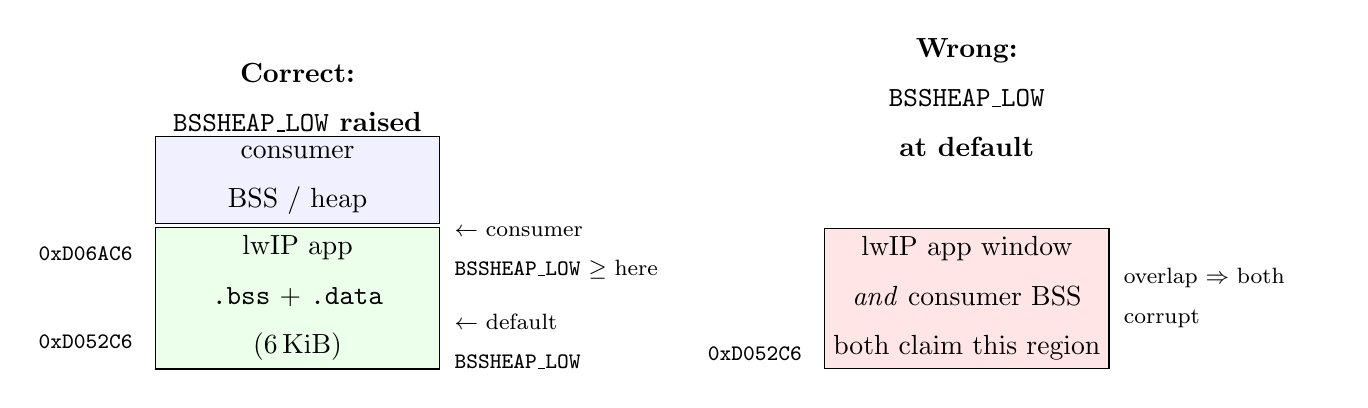
\begin{tikzpicture}[
					font=\footnotesize,
					reg/.style={draw, align=center, text width=3.4cm, inner sep=3pt, minimum height=1.1cm},
					lwip/.style={reg, fill=green!8},
					cons/.style={reg, fill=blue!6},
					bad/.style={reg, fill=red!10, minimum height=1.6cm},
					addr/.style={font=\scriptsize\ttfamily, anchor=east},
					note/.style={font=\scriptsize, anchor=west, text width=3.0cm},
					hdr/.style={font=\footnotesize\bfseries, align=center}
				]
					% addresses increase upward; two independent stacks, well separated
					% ---- LEFT: correct layout ----
					\node[hdr, text width=3.4cm] at (0,3.55) {Correct:\\\texttt{BSSHEAP\_LOW} raised};
					\node[lwip] (L1) at (0,1.0) {lwIP app\\ \texttt{.bss} + \texttt{.data}\\ (6\,KiB)};
					\node[cons, above=1pt of L1] (L2) {consumer\\ BSS / heap};
					\node[addr] at (-1.95,0.45) {0xD052C6};
					\node[addr] at (-1.95,1.57) {0xD06AC6};
					\node[note] at (1.85,1.57) {$\leftarrow$ consumer \texttt{BSSHEAP\_LOW} $\geq$ here};
					\node[note] at (1.85,0.45) {$\leftarrow$ default \texttt{BSSHEAP\_LOW}};

					% ---- RIGHT: broken layout ----
					\node[hdr, text width=3.4cm] at (8.5,3.55) {Wrong:\\\texttt{BSSHEAP\_LOW} at default};
					\node[bad] (R1) at (8.5,1.0) {lwIP app window\\ \emph{and} consumer BSS\\ both claim this region};
					\node[addr] at (6.55,0.3) {0xD052C6};
					\node[note, text width=2.6cm] at (10.35,1.0) {overlap $\Rightarrow$ both corrupt};
				\end{tikzpicture}
				\caption{\footnotesize dylib-mode RAM contract (addresses increase upward). lwIP-CE owns the 6\,KiB window \texttt{0xD052C6}--\texttt{0xD06AC6} for its runtime-initialized \texttt{.bss}/\texttt{.data}. Consumers must set \texttt{BSSHEAP\_LOW}~$\geq$~\texttt{0xD06AC6} (left); leaving it at the toolchain default puts the consumer's BSS on top of lwIP's window and corrupts both (right).}
				\label{fig:bssheap_contract}
			\end{figure}

		\subsection{Validation and Unit Tests}\label{ssec:profiling_unit_tests_ref}
		The project is backed by a deterministic unit test suite that spans the full stack---transport and allocator layers as well as the security-critical cryptographic and parser paths. Tests run on \texttt{CEmu} and are structured around explicit acceptance criteria; where policy requires fail-closed behavior, tests assert rejection rather than silent degradation. (TLS-specific timing and CAVP profiling are treated separately; see Section~\ref{ssec:profiling}.)

		At the transport and allocator level, the Ethernet RX driver is exercised against the real \texttt{usb\_ethernet.c} implementation: ECM frame reception into the RX ring and its drain into lwIP, drain-budget enforcement and backpressure when \texttt{pbuf} allocation fails, NCM NTB parsing across multiple datagrams, and correct USB transfer re-arm state when a transfer fails to schedule. The \texttt{membuffer} allocator is tested across all three buffer classes (ring, pool, file), asserting growth, shrink-hysteresis behavior, max-size rejection, and---under \texttt{BUFFER\_SECURE\_MODE}---automatic zeroization on pop, free, release, and destroy. These tests reach into allocator and driver internal state directly, so a regression in buffering or zeroization is caught rather than masked by surface-level success.

		On the security-critical side, coverage includes truststore integrity verification, certificate-chain trust decisions, RNG initialization/request behavior, parser correctness for ASN.1/X.509/PKCS flows, and expected rejection behavior for malformed or invalid inputs. Tests are built from applicable RFC vectors where available (with RFC and section identifiers recorded in test metadata), and from implementation-directed cases where no official vectors exist.

		Latest unit-test workflow results: \url{https://github.com/cagscalclabs/lwip-ce/actions/workflows/tests.yml}.



		\newpage
		\section{TLS Architecture and Security Model}
	
	This section is not a full TLS implementation guide; it focuses only on platform-specific design choices and any standards deviations that require explicit justification.
	
	\subsection{Threat Model}
	
	Before discussing specific cryptographic constructions and implementation details, it is important to define the threat model under which the lwIP-CE TLS implementation operates. The TI-84+ CE platform was not designed as a secure computing environment, and the security guarantees of this system must therefore be understood within the constraints of the hardware.
	
	This implementation is designed primarily to defend against remote network adversaries while operating on commodity calculator hardware.
	
	\paragraph{Remote Adversaries}
	
	The primary threat model assumes a remote attacker capable of observing, intercepting, and modifying network traffic between the calculator and a remote endpoint. This includes:
	
	\begin{itemize}
		\item Passive network eavesdropping.
		\item Active man-in-the-middle (MITM) attacks.
		\item Malicious or compromised TLS servers.
		\item Malformed or adversarial network inputs intended to trigger parser or protocol failures.
	\end{itemize}
	
	The TLS implementation aims to provide confidentiality, integrity, and endpoint authentication against such adversaries, subject to the correctness of the cryptographic primitives and the trust model described in this document.
	
	\paragraph{Local Adversaries}
	
	A secondary threat model considers attackers with logical access to the device filesystem or software environment. Such attackers may be able to:
	
	\begin{itemize}
		\item Replace application binaries or calculator variables (AppVars).
		\item Modify truststore data or configuration files.
		\item Inspect non-protected memory contents.
	\end{itemize}
	
	Because the platform provides no secure storage primitives or protected execution environment, the system cannot fully defend against a determined local adversary with the ability to modify device storage or execute arbitrary code.
	
	\paragraph{Physical Adversaries}
	
	The TI-84+ CE provides no hardware root-of-trust, secure enclave, or tamper-resistant memory. An attacker with physical possession of the device may be able to:
	
	\begin{itemize}
		\item Extract memory contents through debugging interfaces or external tools.
		\item Observe power, electromagnetic, or timing side channels during cryptographic operations.
		\item Modify stored data or firmware outside the normal execution environment.
	\end{itemize}
	
	Protection against physical attacks and advanced side-channel analysis is therefore outside the scope of this implementation.
	
	\paragraph{Security Goals}
	
	Within the above constraints, the lwIP-CE TLS implementation aims to provide:
	
	\begin{itemize}
		\item Standards-compliant TLS 1.3 handshakes.
		\item Protection of application data against passive and active network attackers.
		\item Robust parsing and rejection of malformed protocol inputs.
		\item Controlled handling of memory and sensitive state where feasible on the platform.
	\end{itemize}
	
	\paragraph{Out-of-Scope Protections}
	
	The system does not attempt to provide:
	
	\begin{itemize}
		\item Hardware-backed key protection.
		\item Resistance to physical device compromise.
		\item Protection against malicious firmware or operating system modification.
		\item Strong resistance to advanced side-channel attacks.
	\end{itemize}
	
	Accordingly, the security properties described in this document should be interpreted as network-level protections operating on top of a fundamentally non-secure hardware platform.
	
	\subsection{HWRNG Design and Entropy Model}
	\label{sec:entropy}
	\label{ssec:entropy}
	
	This section defines the evidence model behind the RNG claims in this document. The objective is to keep distinct:
	\begin{itemize}
		\item design reasoning and implementation intent,
		\item hardware/electrical mechanism,
		\item formal lower-bound analysis, and
		\item empirical calibration from device captures.
	\end{itemize}
	
	Randomness is the foundational security dependency for the TLS stack; if the source is weak, all downstream cryptography is weakened regardless of algorithm choice.
	
	The first technical question, therefore, was whether the TI-84+ CE exposes usable entropy, and if so, how that entropy behaves across hardware revisions. Unlike general-purpose systems, the calculator has very few dynamic entropy sources. Early candidates (such as the \texttt{r} register and cycle counters) were rejected as predictable. The investigation then shifted to hardware-level behavior in unmapped SRAM regions, using community discussion and direct measurement to build a source model that could be tested and bounded.

	This section documents the RNG design rationale and construction, including the statistical and mathematical basis for key decisions, explicit assumptions, identified failure modes, and bounded security estimates. It is not a claim of NIST SP 800-90* compliance or certification. Its purpose is to show that the design was developed against the NIST model and evaluated deliberately rather than implemented ad hoc.

	\paragraph{Entropy Characterization}
	The short answer is yes: the calculator does expose usable entropy, but through a much narrower and weaker physical mechanism than modern general-purpose systems. Cemetech user \textit{Zeroko} summarized the underlying behavior as follows:
	
	\begin{newquote}
		SRAM has a pair of bitlines for each bit of each column address, which are connected to a circuit that tries to make them both be charged to an equal, high level before reading from a memory cell (which partially discharges one of the two) and to a sense amplifier (basically a comparator) to read the resulting state afterward. (There may also be another level of gating between the bitlines and the comparators, but that does not strongly affect the dynamics.) In the unmapped space, there are no memory cells, so the controller equalizes the bitlines however well it does, then does nothing (there being no memory cell to discharge them), then senses which bitline is at a higher level. For some column addresses, this will be heavily biased one way or the other because the pre-charge transistors on the bitlines are too different, while for others, it will be less biased because they are more similar.\\\\
		Another source of non-randomness distinct from the bias is that the bitlines act like capacitors, so precharging only moves their voltage toward the desired level rather than reaching it. This results in a correlation between reads, with the correlation getting weaker with a longer time interval between them and with more intervening reads performed. This is why we cannot just use a von Neumann extractor (which only de-biases) and instead have to do something like XORing many consecutive bits together (which does not fully remove the bias and correlation but can lower it to an undetectable level).  \footnotemark
	\end{newquote}
	\footnotetext{https://www.cemetech.net/forum/viewtopic.php?p=293079\\\textit{Producing crypto-safe randomness on the TI-84+ CE.}}
	
	A clearer restatement followed later in SAX (Cemetech's built-in IRC-style chat room):
	\begin{newquote}
		The circuit involved [in generating entropy] is an SRAM sense amplifier connected to bit lines with no SRAM memory cells at the relevant addresses. So [the circuit] tries to equalize the voltage on the lines (but not quite due to thermal \& noise fluctuations) \& then uses a comparator to decide which is higher (also subject to noise near the decision boundary).
	\end{newquote}

	For readers with a computer engineering background, these mechanics are expected. The key constraint is that, unlike desktop or server platforms that combine many entropy inputs, this platform relies on a single dominant source region with two defining properties:
	\begin{itemize}
		\item Entropy introduced through noise 
		\item Bias and correlation introduced via lazy voltage balancing behavior by the controller
	\end{itemize}
	
	Designing around this required an iterative approach. At the outset, my understanding of entropy modeling and conditioning was limited; through repeated testing, literature review, and community technical feedback, the design converged into a defensible source-selection and conditioning model.
	
	\paragraph{Entropy Tap Selection Model}
	The generator selects an entropy tap via the following algorithm:
	\begin{itemize}
		\item Set monobit-min (current best bit) to range $[512, 1536]$, to effect a worst-case bias of $max(p, 1-p), p \in [0.25, 0.75]$.
		\item Iterate over each bit in the SRAM region defined above, performing a monobit test over 1024 reads for each bit sampled.
		\item Reject any bit whose monobit count does not outperform the current best bit.
		\item If the bit being tested outperforms the current best bit, it becomes the current best bit.
		\item Once the entire region is evaluated, the tap is selected.
	\end{itemize}
	
		The following \textbf{derived assumptions} apply:
		\begin{itemize}
		\item $p \in [0.25, 0.75]$ for the probability of a 1 on the selected raw bit is guaranteed at init/re-init, notwithstanding sudden entropy collapse between health checks. The generator fails outright if no qualifying bit is identified.
		\item Tap selection does not early-exit after finding an acceptable tap; it evaluates the full candidate set, which makes runtime deterministic with respect to scan coverage.
		\end{itemize}
	
	\paragraph{Entropy Tapping Model}
	The generator returns a pseudorandom \texttt{uint64\_t} via the following algorithm:
	\begin{itemize}
		\item Read from the entropy tap into a 119-byte entropy pool.
		\item XOR multiple reads, $n$, into a single composite byte per byte of the entropy pool.
		\item $n$ began as a data-justified heuristic estimate by Zeroko, $k$ was later computed over observable datasets (see Section~\ref{ssec:correlation_calibration}, “Calibrating for Correlation”).
		\item Hash the entropy pool to soften entropy distribution.
		\item Compress digest in blocks to output size.
	\end{itemize}
	
		The following \textbf{derived assumptions} apply:
		\begin{itemize}
			\item Entropy is credited only to the selected source bit; all other bits in each raw byte are treated as zero-entropy in the bound.
			\item XOR conditioning is modeled with effective samples, not independence: \(n_{\mathrm{eff}}=\lfloor n/k \rfloor\).
			\item Conditioning and hashing do not create entropy; they only redistribute/extract available source entropy.
			\item Per-byte min-entropy after conditioning is bounded by \(H_\infty(p_{\mathrm{out}})\), with \(p_{\mathrm{out}}\) derived from the calibrated \(p_{\mathrm{in}}\), \(n\), and \(k\).
			\item Pool-level entropy is bounded as \(m_{\mathrm{eff}} \cdot H_\infty\), where \(m_{\mathrm{eff}}\) uses the same correlation discount model.
			\item Runtime health checks are assumed to detect gross source failure, but short-window entropy collapse between checks remains a residual risk.
		\end{itemize}
		
		\IfFileExists{generated/correlation_data.tex}{
			\input{generated/correlation_data.tex}
		}{
			\newcommand{\CalibRunRows}{test1 & 5 & 0.8867 & 0.4874 & 0.0126 \\ test2 & 5 & 0.8935 & 0.4910 & 0.0090 \\ test3 & 5 & 0.5369 & 0.4997 & 0.0003 \\ test4 & 2 & 0.5861 & 0.4997 & 0.0003 \\ test5 & 5 & 0.8852 & 0.4927 & 0.0073 \\}
			\newcommand{\CalibLineSegments}{\draw[blue!60,opacity=0.8] (1,0.8867) -- (2,0.4874); \draw[blue!60,opacity=0.8] (1,0.8935) -- (2,0.4910); \draw[blue!60,opacity=0.8] (1,0.5369) -- (2,0.4997); \draw[blue!60,opacity=0.8] (1,0.5861) -- (2,0.4997); \draw[blue!60,opacity=0.8] (1,0.8852) -- (2,0.4927);}
			\newcommand{\CalibPointFills}{\filldraw[blue!80] (1,0.8867) circle (0.7pt); \filldraw[blue!80] (2,0.4874) circle (0.7pt); \filldraw[blue!80] (1,0.8935) circle (0.7pt); \filldraw[blue!80] (2,0.4910) circle (0.7pt); \filldraw[blue!80] (1,0.5369) circle (0.7pt); \filldraw[blue!80] (2,0.4997) circle (0.7pt); \filldraw[blue!80] (1,0.5861) circle (0.7pt); \filldraw[blue!80] (2,0.4997) circle (0.7pt); \filldraw[blue!80] (1,0.8852) circle (0.7pt); \filldraw[blue!80] (2,0.4927) circle (0.7pt);}
			\newcommand{\CalibKRows}{test1-bit5 & 0.8867 & 0.4874 & 1.188 \\ test2-bit5 & 0.8935 & 0.4910 & 1.014 \\ test3-bit5 & 0.5369 & 0.4997 & 6.002 \\ test4-bit2 & 0.5861 & 0.4997 & 4.084 \\ test5-bit5 & 0.8852 & 0.4927 & 1.049 \\}
			\newcommand{\CalibKMedian}{1.188}
			\newcommand{\CalibKMean}{2.667}
			\newcommand{\CalibKSigma}{2.033}
			\newcommand{\CalibKQOne}{1.049}
			\newcommand{\CalibKQThree}{4.084}
			\newcommand{\CalibKIQR}{3.035}
			\newcommand{\CalibRangeLow}{1.014}
			\newcommand{\CalibRangeHigh}{6.002}
			\newcommand{\CalibWorkingK}{1.188}
			\newcommand{\CalibBiasRZero}{0.2577}
			\newcommand{\CalibBiasRSeventeen}{0.0059}
			\newcommand{\CalibYTicks}{\foreach \yy/\lbl in {1/1,2/2,3/3,4/4,5/5,6/6}{\draw (0.65,\yy) -- (0.75,\yy);\node[left] at (0.65,\yy) {\scriptsize \lbl};}}
			\newcommand{\CalibKPath}{(1,1.188) -- (2,1.014) -- (3,6.002) -- (4,4.084) -- (5,1.049)}
			\newcommand{\CalibKPointFills}{\filldraw[blue!85] (1,1.188) circle (0.8pt); \filldraw[blue!85] (2,1.014) circle (0.8pt); \filldraw[blue!85] (3,6.002) circle (0.8pt); \filldraw[blue!85] (4,4.084) circle (0.8pt); \filldraw[blue!85] (5,1.049) circle (0.8pt);}
			\newcommand{\CalibXAxisMax}{5.6}
			\newcommand{\CalibXAxisLabel}{5.65}
			\newcommand{\CalibXTicks}{\draw (1,0.55) -- (1,0.65);\node[below] at (1,0.55) {\scriptsize 1}; \draw (2,0.55) -- (2,0.65);\node[below] at (2,0.55) {\scriptsize 2}; \draw (3,0.55) -- (3,0.65);\node[below] at (3,0.55) {\scriptsize 3}; \draw (4,0.55) -- (4,0.65);\node[below] at (4,0.55) {\scriptsize 4}; \draw (5,0.55) -- (5,0.65);\node[below] at (5,0.55) {\scriptsize 5};}
			\newcommand{\CalibXorReads}{17}
			\newcommand{\CalibPoolBytes}{119}
			\newcommand{\CalibOutputBits}{64}
			\newcommand{\CalibPWorst}{0.7500}
			\newcommand{\CalibNeffByte}{14}
			\newcommand{\CalibNeffPool}{1702}
			\newcommand{\CalibPOutByte}{0.49997}
			\newcommand{\CalibPOutPool}{0.50000}
			\newcommand{\CalibMinEntropyBit}{0.99991}
			\newcommand{\CalibMinEntropyOutput}{1.00000}
			\newcommand{\CalibDisplayCount}{5}
			\newcommand{\CalibTotalCount}{5}
			\newcommand{\CalibTruncatedNote}{}
		}
		
	
	
	\subsubsection{Calibrating for Correlation}
	\label{ssec:correlation_calibration}
	This subsection estimates the correlation factor $k$ and the resulting $n_{\text{eff,byte}}$ used by the effective-sample model. We collected 1,179,648 bytes ($\approx$1.2 MB) of source output per device, split evenly across two conditioning modes: no whitening (R0) and 16 XORs (R17). The capture size, though small relative to what some might ask for, was intentionally capped for platform constraints:
	\begin{itemize}
		\item Total calculator storage (RAM + Archive) is roughly 2 MB.
		\item Archive space is partially consumed by resident applications and system artifacts.
		\item SRAM tap behavior is time-varying; long captures increase risk of tap drift during acquisition; continuing collection over re-runs risks choosing different taps, which defeats the purpose.
		\item Pushing capture size substantially higher increases the chance of garbage collection, out-of-memory faults, and collection instability.
	\end{itemize}
	Accordingly, 1.2 MB was selected as a conservative operating point that balances statistical utility against collection reliability. The resulting sample size still provides over 9 million bit observations per mode, sufficient for coarse bias and first-order correlation estimation.
	
	Each mode (R0, R17) was analyzed on computer as an $8\times N$ bit matrix, with each bit column treated as an independent Bernoulli stream. A targeted subset of Dieharder tests was used for coarse non-uniformity screening and repeated across runs for reproducibility checks. Bit-columns were evaluated independently and never concatenated, since mixing columns would invalidate the per-source-bit interpretation. Full local run output is slated for Appendix A and can be extended with community submissions.
	
	Using one best-bit trace per test run (\CalibDisplayCount shown of \CalibTotalCount total) from the dataset:

	\begin{figure}[H]
		\centering
		\begin{minipage}[t]{0.56\textwidth}
			\vspace{0pt}
			\centering
			\scriptsize
			\rowcolors{2}{ltgray}{white}
				\begin{tabularx}{\textwidth}{@{}>{\raggedright\arraybackslash}X*{4}{>{\centering\arraybackslash}X}@{}}
					\toprule
					\rowcolor{gray!18}
					Run & Bit & $p^\star_{R0}$ & $p^\star_{R17}$ & $|p^\star_{R17}-0.5|$ \\
				\midrule
				\CalibRunRows
				\bottomrule
			\end{tabularx}
		\end{minipage}\hfill
		\begin{minipage}[t]{0.42\textwidth}
			\vspace{0pt}
			\centering
				\begin{tikzpicture}[x=2.1cm,y=6.5cm]
					\draw[->] (0.7,0.44) -- (2.35,0.44) node[right] {mode};
					\draw[->] (0.7,0.44) -- (0.7,0.91) node[above] {$p^\star$};
				\foreach \yy/\lbl in {0.5/0.50,0.6/0.60,0.7/0.70,0.8/0.80,0.9/0.90}
				{
					\draw (0.67,\yy) -- (0.7,\yy);
					\node[left] at (0.67,\yy) {\scriptsize \lbl};
				}
				\node[below] at (1,0.44) {\scriptsize R0};
				\node[below] at (2,0.44) {\scriptsize R17};
				
				\CalibLineSegments
				\CalibPointFills
			\end{tikzpicture}
		\end{minipage}
		\vspace{0.1em}
			\caption{\footnotesize{Per-test best-bit progression from raw source (R0) to conditioned output (R17), plotted as $p^\star=\max(p_1,1-p_1)$ so bias direction is folded symmetrically. Each polyline is one test trace from the table above. Full dataset will be available in Appendix 1.}}
		\end{figure}
	\CalibTruncatedNote
	
	On this subset, mean absolute bias contracts from $\CalibBiasRZero$ (R0) to $\CalibBiasRSeventeen$ (R17), consistent with strong whitening under \CalibXorReads-read conditioning.

	This extract, together with the larger dataset, is consistent with the generator constraint: source selection (R0) requires at least one bit no worse than 75/25 bias. Accordingly, the conservative proof domain is set to $p\in[0.5007,\CalibPWorst]$, with bounds evaluated through $\max(p,1-p)$ to cover both bias directions symmetrically.
	
	\[
	k_{\text{eff}}(n)=\min\!\left(\CalibXorReads,\ \max\!\left(1,\ \frac{n\,\ln\!\left|1-2p_{\text{in}}\right|}{\ln\!\left|1-2p_{\text{out}}\right|}\right)\right),\qquad n=\CalibXorReads
	\]
		For implementation-level bounds in this section, $k$ is hard-capped at 17 (the total reads in the 1-read + 16-XOR path) to avoid divergence in the inversion as $p\to0.5$.
	
	Across all \CalibTotalCount $(p_{\text{in}},p_{\text{out}})$ pairs from the dataset (using R0 as $p_{\text{in}}$ and R17 as $p_{\text{out}}$), the raw inversion values are:
	\begin{figure}[H]
		\centering
		\begin{minipage}[t]{0.62\textwidth}
			\vspace{0pt}
			\centering
			\scriptsize
			\rowcolors{2}{ltgray}{white}
			\begin{tabularx}{\textwidth}{@{}>{\raggedright\arraybackslash}X*{3}{>{\centering\arraybackslash}X}@{}}
				\toprule
				\rowcolor{gray!18}
				Run-bit & $p_{\text{in}}$ & $p_{\text{out}}$ & $k_{\text{raw}}$ \\
				\midrule
				\CalibKRows
				\rowcolor{gray!12}
				\bottomrule
			\end{tabularx}
		\end{minipage}\hfill
		\begin{minipage}[t]{0.35\textwidth}
			\vspace{0pt}
			\centering
			\scriptsize
			\rowcolors{2}{ltgray}{white}
			\begin{tabularx}{\textwidth}{@{}>{\raggedright\arraybackslash}X>{\centering\arraybackslash}X@{}}
				\toprule
				\rowcolor{gray!18}
				Metric & Value \\
				\midrule
				Median $k$ & \CalibKMedian \\
				Mean $k$ & \CalibKMean \\
				$\sigma$ (pop.) & \CalibKSigma \\
				Q1 & \CalibKQOne \\
				Q3 & \CalibKQThree \\
				IQR & \CalibKIQR \\
				Defensible range & $[\CalibRangeLow,\,\CalibRangeHigh]$ \\
				\bottomrule
			\end{tabularx}
			\vspace{0.4em}
			\begin{tikzpicture}[x=0.40cm,y=0.28cm]
				\draw[->] (0.7,0.6) -- (\CalibXAxisMax,0.6) node[right] {\scriptsize sample};
				\draw[->] (0.7,0.6) -- (0.7,6.7) node[above] {\scriptsize $k_{\text{raw}}$};
				\CalibXTicks
				\CalibYTicks
				\draw[gray!60,dashed] (0.8,\CalibKQOne) -- (\CalibXAxisMax,\CalibKQOne);
				\draw[gray!60,dashed] (0.8,\CalibKQThree) -- (\CalibXAxisMax,\CalibKQThree);
				\draw[red!70!black,dashed] (0.8,\CalibKMedian) -- (\CalibXAxisMax,\CalibKMedian);
				\draw[blue!70,thick] \CalibKPath;
				\CalibKPointFills
				\node[anchor=west] at (\CalibXAxisLabel,\CalibKQThree) {\scriptsize Q3};
				\node[anchor=west] at (\CalibXAxisLabel,\CalibKMedian) {\scriptsize median};
				\node[anchor=west] at (\CalibXAxisLabel,\CalibKQOne) {\scriptsize Q1};
			\end{tikzpicture}
		\end{minipage}
	\end{figure}

		From these traces, we take $k\in[\CalibRangeLow,\,\CalibRangeHigh]$ as a defensible empirical range and carry forward $k_{median}=\CalibKMedian$ as the central working value.

		For this proof section, the conservative accounting model is:
	\begin{itemize}
		\item only one entropy-bearing bit is credited per pool byte, and
		\item each credited bit is conditioned by \CalibXorReads  reads (1 read + 16 XOR reads).
	\end{itemize}

		With correlation discounting, this gives:
	\begingroup
	\setlength{\abovedisplayskip}{4pt}
	\setlength{\abovedisplayshortskip}{4pt}
	\setlength{\belowdisplayskip}{4pt}
	\setlength{\belowdisplayshortskip}{4pt}
	\vspace{-0.35em}
	\begin{center}
		\begin{minipage}[t]{0.48\textwidth}
			\vspace{0pt}
			\textbf{Per-bit (conditioning depth)}
			\begin{align*}
				n_{\text{eff,byte}} &= \left\lfloor\frac{\CalibXorReads}{k}\right\rfloor
			\end{align*}
		\end{minipage}\hfill
		\begin{minipage}[t]{0.48\textwidth}
			\vspace{0pt}
				\textbf{Across entropy pool}
			\begin{align*}
				n_{\text{eff,pool}} &= \CalibPoolBytes\cdot n_{\text{eff,byte}} = \left\lfloor\frac{\CalibXorReads\cdot\CalibPoolBytes}{k}\right\rfloor
			\end{align*}
		\end{minipage}
	\end{center}
	\vspace{-0.35em}
	\endgroup
	For $k=\CalibKMedian$:
	\begingroup
	\setlength{\abovedisplayskip}{4pt}
	\setlength{\abovedisplayshortskip}{4pt}
	\setlength{\belowdisplayskip}{4pt}
	\setlength{\belowdisplayshortskip}{4pt}
	\vspace{-0.35em}
	\begin{center}
		\begin{minipage}[t]{0.48\textwidth}
			\vspace{0pt}
			\textbf{Per-bit result}
			\begin{align*}
				n_{\text{eff,byte}}&=\left\lfloor\frac{\CalibXorReads}{\CalibKMedian}\right\rfloor=\CalibNeffByte
			\end{align*}
		\end{minipage}\hfill
		\begin{minipage}[t]{0.48\textwidth}
			\vspace{0pt}
				\textbf{Across entropy pool}
			\begin{align*}
				n_{\text{eff,pool}}&=\left\lfloor\frac{\CalibXorReads\cdot\CalibPoolBytes}{\CalibKMedian}\right\rfloor=\CalibNeffPool
			\end{align*}
		\end{minipage}
	\end{center}
	\vspace{-0.35em}
	\endgroup
	
	\paragraph{Min-Entropy}
	\label{ssec:min_entropy}
		We now combine the median correlation coefficient with the worst-case bias assumption $p=\CalibPWorst$ to compute a minimum effective entropy bound.
		
		Using $n_{\text{eff}}$, compute the conditioned Bernoulli parameter per-bit and per-output:
	\begingroup
	\setlength{\abovedisplayskip}{4pt}
	\setlength{\abovedisplayshortskip}{4pt}
	\setlength{\belowdisplayskip}{4pt}
	\setlength{\belowdisplayshortskip}{4pt}
	\vspace{-0.35em}
		\begin{center}
			\begin{minipage}[t]{0.48\textwidth}
				\vspace{0pt}
				\textbf{Per-bit conditioning}
				\begin{align*}
					p_{\oplus}&=\frac{1-(1-2p)^{n_{\text{eff,byte}}}}{2} \\
					p_{\oplus}&=\frac{1-(1-2(\CalibPWorst))^{\CalibNeffByte}}{2} \\
					p_{\oplus}&\approx \CalibPOutByte
				\end{align*}
			\end{minipage}\hfill
			\begin{minipage}[t]{0.48\textwidth}
				\vspace{0pt}
				\textbf{Across entropy pool}
				\begin{align*}
					p_{\oplus}&=\frac{1-(1-2p)^{n_{\text{eff,pool}}}}{2} \\
					p_{\oplus}&=\frac{1-(1-2(\CalibPWorst))^{\CalibNeffPool}}{2} \\
					p_{\oplus}&\approx \CalibPOutPool
				\end{align*}
			\end{minipage}
		\end{center}
		\vspace{-0.35em}
		\endgroup
	
		Now that we have fixed $p_{\oplus}$, we can compute min-entropy over a single bit and over the entire output.
	\begingroup
	\setlength{\abovedisplayskip}{4pt}
	\setlength{\abovedisplayshortskip}{4pt}
	\setlength{\belowdisplayskip}{4pt}
	\setlength{\belowdisplayshortskip}{4pt}
	\vspace{-0.35em}
	\begin{center}
		\begin{minipage}[t]{0.48\textwidth}
			\vspace{0pt}
			\textbf{Per-bit computation}
			\begin{align*}
				H_{\infty}(p)&=-\log_2\!\left(\max(p,1-p)\right) \\
				H_{\infty}(p)&=-\log_2\!\left(\CalibPOutByte\right) \\
				H_{\infty}(p)&\approx \CalibMinEntropyBit
			\end{align*}
		\end{minipage}\hfill
		\begin{minipage}[t]{0.48\textwidth}
			\vspace{0pt}
			\textbf{Across entropy pool}
			\begin{align*}
				H_{\infty}(p)&=-\log_2\!\left(\max(p,1-p)\right) \\
				H_{\infty}(p)&=-\log_2\!\left(\CalibPOutPool\right) \\
				H_{\infty}(p)&\approx \CalibMinEntropyOutput
			\end{align*}
		\end{minipage}
	\end{center}
	\vspace{-0.35em}
	\endgroup
	
	As modeled above, the conditioned output trends to approximately one bit of min-entropy per output bit under the stated assumptions. This satisfies the expected entropy density for secure random artifacts.
	
	The generator’s primitive output width is \texttt{u64}; therefore, larger random artifacts must be produced as sequential blocks, with entropy accounting applied per block and cumulatively.
	
	This is an ultra-conservative reading of the generator, and normal operation is expected to outperform these selected bounds for three reasons:
	\begin{itemize}
		\item The chosen $p$ interval is a worst-case admissible bound. In observed runs, source selection consistently finds at least one bit with lower bias than that bound.
		\item The selected $k$ is the median of empirical estimates; those estimates include upward excursions driven by inversion instability as $p$ approaches $0.5$ (i.e., as $\lim_{p\to0.5}\ln|1-2p|\to-\infty$ in the denominator-sensitive regime).
		\item The proof assigns entropy to only one live bit per source byte. In practice, additional bits may contribute entropy and are also subjected to the same XOR conditioning.
	\end{itemize}
	
	Given this conservative model and empirical calibration, the construction appears suitable for cryptographic randomness generation on this platform, provided it is implemented with proper block-width scaling, reseed and health-check policy, and fail-safe handling on entropy degradation.
	
	\paragraph{Encapsulation}
	\label{ssec:encapsulation}
	
	The generator can be invoked via simple means by simply using the \texttt{tls\_random()} function, or for filling buffers, \texttt{tls\_random\_bytes()}. This allows a user to quickly generate cryptographically suitable randomness without needing to initialize the entire TLS stack. However, this places responsibility for ensuring the continued robustness of the entropy tap on the user, and a function is exposed for this very purpose: \texttt{tls\_rng\_healthcheck()}.
	
	In this mode, entropy output is not pathed through a DRBG, but is instead the direct result of:
	\begin{itemize}
		\item Reading from the entropy tap to a 119-byte entropy pool, with each byte-read being a composite of 17 XOR operations, totaling to 2023 reads for one gathering step.
		\item Running SHA256 over the entropy pool.
		\item XOR compression of the resulting digest into a u64
	\end{itemize}
	This mode relies on the assumption that the tap is stable and that since the user owns the call-stack, they are responsible for ensuring this at the time they read entropy.
	
	Things get a bit more hands-off when the TLS stack is operational given that the stack will occasionally request random bytes invisibly. \texttt{Tls\_init()} enables two timers, one for generator seeding and one for source health checking. Entropy can provided asynchronously by means of a callback-style \textit{entropy request}  (\texttt{tls\_request\_random\_bytes()}). 
		\inputminted[
			breaklines,
			breakanywhere,
			fontsize=\footnotesize,
			firstline=93,
			lastline=93
		]{c}{../../src/tls/includes/random.h}
	This:
	\begin{itemize}
		\item Registers a request for random bytes, a buffer to return those bytes into, and a callback to run when the request completes.
		\item If \texttt{blocking=true}, execution halts until enough entropy is returned to fill the request.
		\item If \texttt{blocking=false}, execution returns to the caller immediately; the callback function fires when the request is fullfilled.
	\end{itemize}
	
		While being used within TLS, entropy is returned through a SHA-256 DRBG serviced by a 50\,ms request timer. On each timer cycle, the RNG path behaves as follows:
		\begin{itemize}
			\item A health-check gate runs first. If source health fails, the gather step aborts and no new DRBG material is accepted for that cycle.
			\item One \texttt{tls\_random()} value (8 bytes) is collected.
			\item \textbf{If the DRBG is not yet instantiated}: those 8 bytes are appended to seed material. Once 32 bytes total are accumulated, the DRBG state is instantiated as \texttt{SHA256(seed\_material)}.
			\item \textbf{If the DRBG is already instantiated}: the new 8-byte sample is mixed by reseeding the state with a SHA-256 update over current state, entropy chunk, and counter.
			\item An entropy budget is credited by 8 bytes each successful gather, capped at 32 bytes.
			\item Active requests are fulfilled from DRBG output only when budget is available; output decrements the budget by the number of bytes returned.
		\end{itemize}
		In blocking mode, \texttt{tls\_request\_random\_bytes()} runs this same gather/fulfill loop synchronously until complete (or retry limit). In non-blocking mode, requests are queued and completed by the timer path.
		
		Additionally, a RNG source health check is also serviced by a 30s timer that runs the following statistical analysis:
		\begin{itemize}
			\item Request 32 random bytes through \texttt{tls\_random()}. Note that we are not using DRBG-conditioned output.
			\item If sample matches last sample, fail health check.
			\item Test monobits (total \texttt{1} bits across sample). If outside range $[88, 168]$, fail health check.
			\item Test max equal byte run. If max run exceeds 4, fail health check.
		\end{itemize}
		These tests and sample sizes represent a tradeoff between test quality and the calculator's available computation.
		
		If quick statistical testing demonstrates that the source has degraded beyond acceptable levels, the generator initialization function is called, which should cause a new source to be selected. Given the abstraction between tap, the entropy pool, and the DRBG, choosing a new entropy tap is invisible and does not impact upstream state.

	\subsection{Certificate Chain Trust Model}
	A core requirement for Internet security is authenticating that the remote endpoint is actually the party it claims to be. In TLS, that assurance is normally derived from certificate-chain validation against a trust anchor.
	
	On this platform, however, certificate handling introduces three practical constraints:
	\begin{itemize}
		\item Certificate chains can be large (often multiple kilobytes), which is expensive relative to available heap.
		\item Full-path X.509 processing and repeated signature checks are computationally heavy on the CE.
		\item As with the RNG capture constraints discussed earlier, the CE does not have sufficient storage budget for a desktop-scale trust store.
	\end{itemize}
	We needed a trust model that remained defensible for the intended use case while still allowing the calculator to complete a handshake without experiencing a nuclear meltdown in its CPU. We settled on a signed SPKI-pinning trust model, combined with the mandatory TLS 1.3 \texttt{CertificateVerify} check for live proof-of-possession. This approach is intentionally narrower than a full desktop-class WebPKI verifier: the tradeoff is reduced processing and memory pressure in exchange for an explicit, managed trust boundary defined by the shipped truststore.

	\paragraph{Trust Store}
	Trust is expressed as pinned \texttt{SubjectPublicKeyInfo} (SPKI) identities in a signed truststore, shipped as a compact platform-specific bundle. Its generation, on-device format, and lifecycle are detailed in the next section.

	\paragraph{CertificateVerify}
	SPKI-pinning establishes that the chain the server presented contains a CA we recognize, but it does not on its own prove that the entity we are speaking with controls the leaf private key. A network attacker holding only the leaf certificate---which is public---would otherwise pass the pin check. TLS 1.3's \texttt{CertificateVerify} message closes that gap: the server signs a digest of the handshake transcript with its leaf private key. We require this message and verify it on every full handshake.

	The implementation is restricted to \texttt{rsa\_pss\_rsae\_sha256} with a leaf RSA modulus between 1024 and 2048 bits. Servers selecting \texttt{ecdsa\_secp256r1\_sha256}, the wider RSA-PSS hash variants, or RSA-PKCS1 (which RFC~8446 §4.4.3 forbids in \texttt{CertificateVerify} regardless) are rejected with a fatal \texttt{decrypt\_error} alert. Support for \texttt{ecdsa\_secp256r1\_sha256} is planned.

	\paragraph{Certificate Chain Parsing}
	When operating as a client and processing the TLS \texttt{Certificate} message, the implementation parses the X.509 chain and evaluates each certificate as follows:
	\begin{enumerate}
		\item Extract \texttt{SubjectPublicKeyInfo} and compute its SHA-256 digest.
		\item Verify required CA constraints (\texttt{BasicConstraints cA=TRUE}; if \texttt{KeyUsage} is present, \texttt{keyCertSign}).
		\item Check whether the digest matches a pinned truststore entry, and where time is sane, enforce validity-window and owner/issuer metadata checks on a match.
	\end{enumerate}
	The chain is accepted only if at least one CA-capable certificate satisfies the trust and constraint checks above \emph{and} the leaf's \texttt{CertificateVerify} signature verifies (per the previous paragraph). Otherwise the handshake is terminated. The on-device truststore format consulted in step~3 is specified in the next section.

	\subsection{Trust Store Generation and Specification}

	\paragraph{Generation}
	The truststore is generated by a scheduled GitHub Actions workflow (quarterly) and published as a signed TI AppVar (\texttt{.8xv}) for device deployment. Conceptually, it serves the same role as an OS trust-anchor bundle, but in a compact, platform-specific format.
	The \texttt{Store Version} field is a binary schema compatibility contract, not a content revision marker. It is incremented only when serialization/parsing semantics change in a way that affects decoding. Routine truststore content updates, naming changes, and signer-key rotation do not require a version increment.

	The workflow:
	\begin{enumerate}
		\item Scans common CA-certificate locations on the runner (for example \texttt{/etc/ssl/certs}) and collects parseable trust anchors.
		\item Extracts the following metadata from each certificate:
		\begin{itemize}
			\item The \texttt{SubjectPublicKeyInfo} field
			\item The issuer and owner IDs
			\item The expiry timestamps (not-before, not-after)
		\end{itemize}
		\item Serializes a binary truststore with the following layout:
		\begin{figure}[H]
			\centering
			\scriptsize
			\rowcolors{2}{ltgray}{white}
			\begin{tabularx}{0.92\textwidth}{@{}>{\raggedright\arraybackslash}X>{\centering\arraybackslash}m{2.4cm}>{\raggedright\arraybackslash}X@{}}
				\toprule
				\rowcolor{gray!18}
				Field & Size & Notes \\
				\midrule
				Signature Field & 256 bytes & File signature / authenticity block \\
				Store Version & 2 bytes & Truststore schema version \\
				Created Timestamp & 4 bytes & Build timestamp \\
				Cert Entry Count & 2 bytes & Number of certificate records \\
				\rowcolor{gray!22}
				\multicolumn{3}{@{}l@{}}{\textbf{Per-certificate record (repeated \texttt{Cert Entry Count} times)}} \\
				Owner Id & 32 bytes & Truncated if source identifier exceeds 32 bytes \\
				Issuer Id & 32 bytes & Truncated if source identifier exceeds 32 bytes \\
				Not-Before & 4 bytes & Validity start timestamp \\
				Not-After & 4 bytes & Validity end timestamp \\
				SHA-256 SPKI & 32 bytes & Digest of SubjectPublicKeyInfo \\
				EOF & -- & End of file \\
				\bottomrule
			\end{tabularx}
		\end{figure}
		\item Signs the truststore bytes from \texttt{Store Version} through \texttt{EOF} using RSA-2048 PSS-SHA-256 and writes the signature into \texttt{Signature Field}.
		\item Stores the signing key in GitHub Secrets, materializes it only in runner temp storage for signing/verification, then deletes it (including \texttt{shred} cleanup).
		\item Converts the binary store to TI AppVar format (\texttt{.8xv}) via \texttt{convbin}.
		\item Publishes the resulting AppVar as the \texttt{truststore-latest} release artifact.
		\item Links validation at runtime by shipping the corresponding public verification key within lwIP's truststore module.
	\end{enumerate}
	
	Truststore age is currently a soft-fail signal, not an enforced rejection condition. A stale store can trigger warning behavior, but does not by itself block use of an otherwise valid signed truststore. Age checks are meaningful only when time is sane, which requires either (1) a valid local clock state, or (2) a functioning NTP path.
	
	Algorithm agility is version-gated. The current format uses RSA-2048 PSS-SHA-256 for truststore signatures; future signature-scheme migrations are expected to ship behind an explicit format/version transition plus corresponding verifier update.

	\paragraph{Runtime Initialization}
	When the TLS module initializes, it also initializes the truststore, which performs (1) signature verification of the truststore against the embedded public verification key, and (2) schema/version compatibility checks against the version expected by lwIP. If truststore initialization fails, TLS client connections are refused.

	\paragraph{Compromise and Revocation}
	If the truststore signing key is suspected or confirmed compromised, the incident response is:
	\begin{enumerate}
		\item Revoke and replace the compromised signing key.
		\item Regenerate the truststore under the replacement key.
		\item Publish a new lwIP release embedding the replacement public verification key.
		\item Publish a security advisory across project channels (GitHub, Discord, and community forums).
	\end{enumerate}

	
	\subsection{Profiling}\label{ssec:profiling}

	Alongside the stack-wide unit tests described in Section~\ref{ssec:profiling_unit_tests_ref}, this section covers the TLS-specific, profiling-oriented validation layer. Where unit tests verify functional correctness, safety checks, and regression resistance for module behavior, profiling tests characterize timing stability, performance behavior, and platform-dependent variance under controlled workloads.

	Profiling tests are intentionally separated from strict correctness gating. Their role is to quantify behavior, not merely assert it. In particular, timing-oriented tests evaluate differential behavior across input classes and report whether observed variance remains within calibrated bounds. Because timing consistency evidence is environment-sensitive, profiling outcomes are interpreted as indicators and trend signals rather than formal proofs.
	
	\subsubsection{Timing Analysis Profiler}
	The primary profiling module, \texttt{tls\_timing}, uses robust per-primitive calibration instead of a fixed global cycle limit. For each primitive, repeated samples are collected on a calibration class (``same input'', currently the best-case class), yielding cycle samples $\{T_1,\dots,T_n\}$. The following robust statistics are then computed:
	
	\begin{align*}
		m &= \operatorname{median}(T_1,\dots,T_n),\\
		\operatorname{MAD} &= \operatorname{median}\left(\left|T_i - m\right|\right),\\
		\sigma_{\text{robust}} &= 1.4826 \cdot \operatorname{MAD}.
	\end{align*}
	
	For each tuning constant $c$, the accepted cycle deviation is:
	\begin{align*}
		\Delta_c = \max\!\left(c,\; c\cdot \sigma_{\text{robust}}\right).
	\end{align*}
	
	Two $c$ modes are reported for every primitive:
	\begin{itemize}
		\item \textbf{Standard mode}: $c=6$ (used for pass/fail gating in CI).
		\item \textbf{Rigorous mode}: $c=4$ (reported for additional strictness, not current gate criterion).
	\end{itemize}
	
	Each primitive is then evaluated across input classes (best, worst, random, edge), defined:
	\begin{itemize}
		\item \textbf{Best-Case}: Input is filled with $0x00$.
		\item \textbf{Worst-Case}: Input is filled with $0xFF$.
		\item \textbf{Random}: Input is filled with pseudo-randomness.
		\item \textbf{Edge-Case}: First half of the input is filled with $0x00$ and the second half is filled with $0xFF$.
	\end{itemize}
	
	For each class, the reported statistics include class median deviation from the calibration median and exceedance rate (percentage of samples where $|T_i-m|>\Delta_c$). A differential failure is flagged when separation from calibration exceeds the accepted deviation with directionally consistent behavior across at least a three-quarters majority of samples.	
	
	Each unit is sampled $50$ times, where each sample is a composite of repeated executions selected by algorithm runtime class: fast units use $64$ repetitions, medium units use $16$, and slow units use $2$. This batching further suppresses class-independent timing jitter.

	Latest timing-profiler workflow results: \url{https://github.com/cagscalclabs/lwip-ce/actions/workflows/timing.yml}.

	\subsubsection{CAVP Validation}

	Formal cryptographic certification depends not only on algorithm behavior, but also on implementation context, build process, operating environment, and hardware security properties. Because this stack runs as calculator application code on hardware without a secure execution environment or certified key-storage boundary, it is not presented as a formally certified cryptographic module.

	
	Instead, the project demonstrates algorithmic correctness against NIST CAVP-published response files and compatible generated reference vectors. The CAVP workflow downloads the relevant NIST \texttt{.rsp} vector archives for supported primitives and selects 16 random samples per primitive on each run. For primitives without compatible CAVP response files, vectors are generated during the workflow with \texttt{python3-cryptography} using the relevant RFC-defined algorithm parameters. If NIST resources are unavailable, the workflow uses the cached CAVP archives from a previous successful run; if neither the source archive nor cache is available, validation fails closed.

	The selected samples are packaged into the \texttt{CAVPIN} AppVar and transferred to the emulator, where the calculator-side runner dispatches each vector to the corresponding implementation. Results are written into \texttt{CAVPOUT}, transferred back to the runner, and parsed against the expected outputs produced from the NIST or \texttt{python3-cryptography} reference material. This provides randomized regression coverage and evidence from CAVP-derived vector checks, without representing a formal CAVP submission or certification.

	\paragraph{Round-trip pipeline}: The reason for the AppVar hand-off is that the implementation under test only exists on the calculator --- the same eZ80 binary that ships, not a host re-build --- so the vectors have to travel to the device and the answers have to travel back. The pipeline has four stages. \emph{(1) Serialization}: the host harness encodes the selected vectors (inputs, keys, IVs, and the metadata identifying which primitive and operation each belongs to) into the \texttt{CAVPIN} AppVar, a flat binary layout the on-device runner can walk without a parser. \emph{(2) On-device execution}: \texttt{CAVPIN} is loaded onto the emulator, the runner reads each record, calls the real lwIP-CE implementation, and appends the computed output to the \texttt{CAVPOUT} AppVar --- the device never sees the expected answers, so it cannot accidentally echo them. \emph{(3) Exfiltration}: \texttt{CAVPOUT} is pulled back off the emulator to the host. \emph{(4) Comparison}: the host parses \texttt{CAVPOUT} and checks each computed value against the reference output it withheld in stage~1, byte-for-byte. A mismatch on any sample fails the run and names the offending primitive and vector index, so a regression points at a specific algorithm rather than a vague ``CAVP failed.'' Keeping the reference answers exclusively on the host side is deliberate: it ensures the device is genuinely computing the result, not transporting it.

	\paragraph{Exclusions}: RSA-PSS vectors are generated with \texttt{python3-cryptography} because this implementation fixes $e=65537$, while the available NIST PSS response files do not provide a compatible fixed-exponent set. X25519 vectors are also generated with \texttt{python3-cryptography}, supplemented by RFC 7748 vectors, because CAVP does not publish X25519 coverage for this use case.

	Latest CAVP-validation workflow results: \url{https://github.com/cagscalclabs/lwip-ce/actions/workflows/cavp.yml}.
	
\begin{center}
\rule{0.7\linewidth}{0.2pt}
\end{center}

	The workflow pipeline runs these layers independently so long-running profiling does not block deterministic unit validation. Unit results provide hard regression gates; profiling results provide ongoing security/performance telemetry and flag areas requiring deeper analysis. Together, they form a practical validation model for a constrained platform: strict correctness checks where determinism is expected, and measured characterization where hardware/runtime noise is unavoidable.
	
	As with the rest of this document, these tests support engineering confidence and change control, but do not constitute external certification. Their purpose is to make assumptions explicit, catch regressions early, and provide reproducible evidence for design and security claims. The timing framework is intended to detect input-dependent regression and structural timing drift, not to serve as a formal leakage proof under adversarial averaging models.

	\subsubsection{Continuous Integration}
	\label{ssec:ci}

	Test execution is structured for reviewability rather than just pass/fail signaling. Four self-audit workflows run on every push via GitHub Actions --- the deterministic unit suite (\texttt{tests.yml}), CAVP-vector validation (\texttt{cavp.yml}), the differential timing profiler (\texttt{timing.yml}), and static analysis (\texttt{sast.yml}) --- each producing a self-contained job summary intended to be readable as an audit artifact without reference to source. (A fifth workflow, \texttt{build.yml}, simply confirms the project compiles, and is not part of the validation set.)

	The unit-test job summary surfaces, for each unit, the RFC and section identifier the tests are derived from (recorded as part of test metadata at authoring time). On failure, the specific RFC test vector that diverged is reported rather than just the failing unit, so a reader can immediately locate the corresponding normative reference. The differential timing profiler emits a per-build chart of class-versus-calibration deviations directly into the job summary, alongside per-primitive median and exceedance-rate tables, so trend drift across builds is visible without downloading raw logs.

	\paragraph{How to read a run (for external reviewers)}: open the Actions tab at the link below and select a commit; the four self-audit workflows appear as separate checks. A green run means every gate passed for that commit; the substance is in each workflow's \emph{job summary}, which is written to be read on its own without cloning the repository. For \textbf{unit tests}, the summary lists each unit with its governing RFC/section, and on failure names the exact diverging vector --- so a reviewer confirms not just \emph{that} a primitive passed but \emph{against which normative reference}. For \textbf{CAVP}, the summary reports per-primitive pass counts over the randomly sampled vectors, with any mismatch identified by primitive and vector index. For \textbf{timing}, the summary embeds the per-primitive deviation chart and the median/exceedance tables; a reviewer looks for all-green rows and near-zero median deviation, and treats any red row or elevated exceedance rate as a flagged item rather than an automatic failure (timing evidence is interpreted as a trend signal, per the profiling discussion above). For \textbf{SAST}, the summary lists Semgrep findings scoped to code the project added or changed relative to upstream lwIP, so review effort lands on new surface rather than the inherited base. Because every summary is self-contained and regenerated on each push, a reviewer can audit the current state of any claim in this document directly from the latest run, without trusting a cached artifact or re-deriving it locally.

	The latest workflow runs are accessible at \url{https://github.com/cagscalclabs/lwip-ce/actions}.

	One deliberate exclusion is worth documenting: the RNG unit tests are not part of the automated CI pipeline. The CI environment executes against \texttt{CEmu}, whose SRAM emulation is deterministic and does not reproduce the physical bitline behavior the entropy source depends on. Emulated RNG output is therefore statistically meaningless for the purposes of this implementation, and incidental emulator-quirk failures during source selection would block unrelated regression gates. RNG validation is instead performed against hardware captures, following the protocol described in Section~\ref{ssec:contributing_data}.

	\subsubsection{Community Data Contributions}
	\label{ssec:contributing_data}

	Two of the analyses in this document --- the empirical correlation calibration in Section~\ref{ssec:correlation_calibration} and the differential timing characterization above --- benefit materially from broader hardware coverage than any individual developer can produce. The TI-84+ CE has gone through several hardware revisions over its production lifetime, and physical-source behavior (in particular the SRAM bitline characteristics underlying the entropy tap) is not guaranteed to be uniform across them. Community-contributed captures expand the empirical envelope rather than re-validate the existing bound: each submission adds coverage for a device class the project's own benches do not include.

	\paragraph{What to capture}
	Two on-device tools produce the submission artifacts:
	\begin{itemize}
		\item \textbf{RNG calibration capture.} Produces a series of AppVars, half for raw source output (R0) and half for 16-XOR conditioned output (R17). The output is sharded across multiple AppVars because individual AppVar size and on-device pagination limits prevent emitting a single contiguous file. A companion Python script (in \texttt{docs/whitepaper/scripts/}) parses the submitted AppVars, treats each byte as eight independent bit streams (bit position 1 across all bytes is one stream, bit position 2 another, and so on), and performs per-stream Bernoulli analysis. This per-bit-column treatment is the empirical mirror of the proof's accounting assumption in Section~\ref{ssec:entropy} that credits at most one entropy-bearing bit per source byte.
		\item \textbf{Differential timing capture.} Produces a structured log file using a \texttt{key=value} record format. Each unit's calibration class and per-class results are emitted with explicit denotation so the upstream analysis can locate each unit and its associated measurements by regular expression. The log can be exfiltrated via standard AppVar transfer.
	\end{itemize}

	\paragraph{Device identification}
	Contributions are most useful when accompanied by enough device metadata to locate the submission within the broader sample population. At minimum:
	\begin{itemize}
		\item Hardware revision (visible on the back-label sticker or via \texttt{[mode]} $\rightarrow$ \texttt{[about]}).
		\item Operating system version.
		\item Boot code version, where reported by the device.
	\end{itemize}
	Contributors who are unsure which revision they hold are encouraged to submit anyway with whatever metadata they can identify; the project can usually disambiguate from the supplied OS and boot-code strings.

	\paragraph{How to submit}
	Submissions can be sent via either channel below:
	\begin{itemize}
		\item Project Discord: \url{https://discord.gg/CtEq3rXZGJ} --- a dedicated channel exists for capture submissions and questions about the protocol.
		\item Direct email: \texttt{info@cagscalclabs.net} --- preferred when attaching large AppVar bundles.
	\end{itemize}
	The capture tool itself, its source, and the parsing scripts are versioned within this repository; contributors are asked to record which tool version produced their submission so the analysis pipeline can account for any schema changes between releases.

	\paragraph{Privacy and licensing}
	The project does not collect personally identifying information from contributors and does not maintain an attribution roster for submitted captures. This is a deliberate privacy-by-design choice: the community includes minors, and the analytical value of a capture is determined entirely by the device metadata accompanying it (hardware revision, OS version, boot code), not by the identity of the submitter. Captures are processed and incorporated into the published dataset under the project's existing license; once accepted, a capture is not retraceable to its submitter through any project-controlled record. Contributors who wish to be visible may of course identify themselves publicly on Discord or in GitHub discussions, but the project itself maintains no such linkage.

	\subsection{Profiling and Mitigating Platform Security Limitations}
	
	\subsubsection{The TI-84+ CE Hardware Security Profile}
	The TI-84+ CE hardware security profile is sufficiently limited that, while drafting this section, I considered leaving it blank; doing so would not materially change the conclusion.
	
	The TI-84+ CE provides no meaningful hardware root-of-trust, no secure enclave, and no robust anti-tamper boundary. Accordingly, all software security claims in this document are explicitly bounded by that platform reality. 
	
	\textbf{Profile Characteristics}
	\begin{itemize}
		\item The platform is built around a Zilog eZ80-class CPU (24-bit addressing mode, 48\,MHz class operation), optimized for calculator workloads rather than secure key custody or trusted execution.\footnote{\url{https://ce-programming.github.io/toolchain/static/hardware.html}}
		\item The platform does not expose a hardware secure enclave, TPM-equivalent, or other dedicated primitive for sealing long-term private key material in user-space workflows.
		\item Memory and storage interfaces are not designed as tamper-resistant boundaries against a local adversary with physical control of the device and transfer path.
		\item Security-sensitive software therefore operates as a best-effort hardening layer over commodity calculator hardware, not as a hardware-backed trust anchor.
		\item Runtime checks that depend on wall-clock time (for example certificate validity windows or truststore age warnings) are only as reliable as the device clock state or external synchronization path.
	\end{itemize}
	
	From this profile, the implementation \textbf{cannot fully defend against}:
	\begin{itemize}
		\item Physical side-channel leakage (power/EM/thermal) from the device during cryptographic operation.
		\item Local code-execution adversaries that patch binaries, bypass integrity checks, or tamper with persistent containers (for example AppVars).
		\item Offline extraction or modification of unsealed keying material and trust artifacts when the device/storage path is under attacker control.
	\end{itemize}
	
From this profile, the implementation \textbf{can partially mitigate}:
\begin{itemize}
	\item Host-assisted memory observation during active cryptographic transforms (for example side-loading plus memory mapping).
	\item Leakage of secrets or intermediate plaintext $\leftrightarrow$ ciphertext transform state in stack and allocated buffers, through explicit zeroization and guarded handling.
\end{itemize}
These mechanisms are implemented via the \textbf{cryptoguard} wrapper detailed in the next section.
	
	\subsubsection{Cryptoguard Wrapper}
	In an effort to provide modest defense against host-assisted memory observation and leakage of secrets/plaintext, we implemented a \texttt{cryptoguard} module. This module provides wrapper functions around security-sensitive contexts. The module:
	\begin{itemize}
		\item Saves the current interrupt state, then disables system interrupts. This reduces the opportunity for host-assisted observation during sensitive operations, since USB activity handling depends on interrupt-driven processing. On exit, the prior interrupt state is restored.
		\item Clears stack memory from the current stack location up to the configured stack top before returning to the caller. This reduces residual exposure of stack-allocated buffers and intermediate values after sensitive routines complete.
	\end{itemize}
	
	The current cryptoguard wrapper implementation is included below directly from source:
	
	\IfFileExists{../../src/tls/core/share/crypto_guard.s}{
		\inputminted[
			breaklines,
			breakanywhere,
			fontsize=\scriptsize
		]{tasm}{../../src/tls/core/share/crypto_guard.s}
	}{
		The file \texttt{../../src/tls/core/share/crypto\_guard.s} was not found at build time.
	}
	
\textbf{Additional Implemented Security Mechanisms}
\begin{itemize}
	\item \texttt{tls\_secure\_memzero()}: A secure zeroization routine intended to avoid compiler elimination of memory-clearing operations. Unlike a plain \texttt{memset()}, it uses \texttt{volatile}-qualified access so clearing side effects are preserved during optimization.
	\item \textbf{Secure Membuffer Contexts}: As noted in the allocator section, a \texttt{membuffer} created with \texttt{BUFFER\_\allowbreak SECURE\_\allowbreak MODE} applies automatic zeroization in key lifecycle paths:
	\begin{itemize}
		\item when \texttt{free()} is called on pool-allocated blocks;
		\item when bytes are popped from a ring buffer;
		\item in dynamic mode, when the allocation shrinks (the released region is zeroed).
	\end{itemize}
\end{itemize}

When evaluated in unison, these mechanisms provide best-effort memory sanitization across allocation, use, and teardown paths, reducing residual plaintext/key exposure without claiming complete protection against a local or physical adversary.

	
		\newpage
		
		\section{Conclusion}
		This work demonstrates that a modern TCP/IP stack with TLS support can be adapted to the TI-84+ CE class of hardware when the design is shaped around the platform rather than merely compressed to fit it. More broadly, it is an existence proof for a class of device most would write off entirely: a single-core processor in the low tens of megahertz, with no MMU, no hardware cryptographic acceleration, no secure element, and a memory budget measured in kilobytes can still host an interoperable TLS~1.3 client against the live internet --- provided the constraints are treated as first-class design inputs rather than obstacles to paper over. The resulting system combines USB CDC Ethernet transport, lwIP protocol handling, memory-pressure-aware buffering, a resident application call model, and a constrained TLS 1.3 implementation into a coherent network stack for a device with severe memory, timing, and security limitations.
		
		The central engineering result is not that the TI-84+ CE can be made equivalent to a desktop or server environment. It cannot. The platform lacks a hardware root of trust, secure key storage, preemptive multitasking, and the memory budget normally assumed by contemporary networking and cryptographic software. The relevant result is narrower and more useful: with explicit boundaries, conservative assumptions, and targeted validation, the platform can support interoperable secure-client workflows and provide a practical foundation for calculator-native networked applications.
		
		Several design choices carry that result. The USB Ethernet driver limits scope to CDC ECM/NCM behavior that can be made reliable on the device. The membuffer layer makes allocation pressure visible and gives ingress paths a way to degrade predictably. The RNG model treats the hardware entropy source as something to be measured, conditioned, and health-checked rather than assumed. The truststore design replaces desktop-scale WebPKI expectations with a signed, compact, platform-specific trust boundary. The TLS implementation and profiling suite then build on those constraints with explicit tests, timing telemetry, and failure behavior.

		The four self-audit workflows described in this document --- deterministic unit testing, CAVP-vector validation, differential timing analysis, and static analysis (SAST) --- are not isolated test jobs but a single, deliberately layered \emph{pre-audit validation pipeline}. Unit testing establishes functional correctness and fail-closed behavior against RFC- and CAVP-derived vectors; CAVP validation independently confirms that the shipping on-device binary computes standard algorithm outputs correctly, end to end; differential timing analysis characterizes the constant-time properties that functional tests cannot see; and SAST (Semgrep) statically scans the project's own additions against upstream lwIP for unsafe patterns, so review attention is focused on changed code rather than the inherited base. Each runs on every push and emits a self-contained, source-independent job summary. Collectively they are intended to do the preparatory work a formal third-party audit would otherwise start from scratch: they make the project's correctness, timing, and code-quality claims continuously reproducible, machine-checked, and legible to an external reviewer, so that an audit can begin from evidence rather than assertion. That this depth of standing validation is achievable on a calculator is itself part of the result.
		
		At the same time, this implementation should be understood as a constrained engineering artifact, not as a certified cryptographic module. It has not undergone formal third-party audit or certification, and its security claims are bounded by the hardware profile described in this document. Local physical attackers, compromised binaries, and side-channel observation remain outside the set of problems this project can fully solve. The mitigations provided here are best-effort hardening measures, not a substitute for secure hardware.
		
		The practical value of lwIP-CE is therefore twofold. First, it provides a usable networking and TLS substrate for calculator programs that would otherwise have no realistic path to modern internet protocols. Second, it documents the tradeoffs required to bring such a stack to a nontraditional embedded platform. Future work should focus on external review, continued interoperability testing, broader device sampling for entropy behavior, and continued tightening of the TLS and truststore policy surface.
		
		Within those limits, lwIP-CE shows that secure embedded networking on deeply constrained hardware is not a matter of pretending the constraints do not exist. It is a matter of making them explicit, measuring what can be measured, and designing each layer so that the system fails visibly and predictably when those constraints are exceeded.
		

	\newpage
	\section{Contributions, References, and AI-Assisted Tooling Disclosure}\small
	\subsection{Contributions}
	Special thanks to the following individuals who contributed materially to the project:
	\begin{table}[htbp]
		\centering
		\renewcommand{\arraystretch}{1.12}
		{\footnotesize
			\begin{tabularx}{\textwidth}{p{0.20\textwidth} p{0.8\textwidth}}
			\hline
			\textbf{Role} & \textbf{Contributor(s)} \\
			\hline
			Lead Developer & Anthony Cagliano \\
			C $\rightarrow$ eZ80 & Adam Beckingham \\
			Entropy Analysis & Zeroko \\
			modexp\_2048 & jacobly \\
			x25519 & Peter Tillema (PT\_) \\
			fasmg to GNU migration & TIny\_Hacker \\\hline
			Other Contributions (Info, Optimizations, Supporting Algorithms) &  \begin{tabular}[t]{p{0.2\textwidth} p{0.2\textwidth} p{0.2\textwidth}}
				jacobly & calc84maniac & Zeroko \\
				John Caesarz & MateoC & 
			\end{tabular} \\\hline
			Testers &   \begin{tabular}[t]{p{0.2\textwidth} p{0.2\textwidth} p{0.2\textwidth}}
				Alessio &
			\end{tabular} \\\hline
			Donations &   \begin{tabular}[t]{p{0.2\textwidth} p{0.2\textwidth} p{0.2\textwidth}}
			\end{tabular} \\
			\hline
		\end{tabularx}
		}
	\end{table}

	\subsection{References}
	\begin{table}[htbp]
		\centering
		\renewcommand{\arraystretch}{1.12}
		{\footnotesize
		\begin{tabularx}{\textwidth}{p{0.20\textwidth} p{0.5\textwidth} p{0.3\textwidth}}
			\hline
			\textbf{Source} & \textbf{Use in This Project} & \textbf{Reference} \\
			\hline
			B-Con \texttt{crypto-algorithms} & Ported reference implementation for AES block/key-schedule routines and SHA-256 core hashing primitives. & \url{https://github.com/B-Con/crypto-algorithms/} \\
			tiny-ECDH-c & Reference ECDH implementation basis. & \url{https://github.com/kokke/tiny-ECDH-c} \\
			lwIP (upstream) & Upstream TCP/IP stack source lineage used as networking foundation and reference baseline. & \url{https://savannah.nongnu.org/projects/lwip/} \\
			RFC 4868 & HMAC-SHA-256 construction details and test-vector guidance. & \url{https://datatracker.ietf.org/doc/html/rfc4868} \\
			NIST SP 800-38D & AES-GCM mode specification and implementation details. & \url{https://nvlpubs.nist.gov/nistpubs/Legacy/SP/nistspecialpublication800-38d.pdf} \\
			NIST SP 800-90 Series & RNG design/specification guidance (DRBG and entropy-source validation criteria). & \url{https://csrc.nist.gov/projects/random-bit-generation/sp-800-90} \\
			Shemanske, \textit{Modern Cryptography and Elliptic Curves} & Elliptic-curve background and conceptual reference. & Book \\
			\hline
		\end{tabularx}
		}
	\end{table}

	\subsection{AI-Assisted Tooling Disclosure}
	AI-assisted tooling was involved in limited engineering and drafting workflows. AI assistance was used for tasks such as:
	\begin{itemize}
		\item Code quality analysis, alongside SAST and manual review.
		\item Initial scaffolding and review of portions of the TLS handshake control flow.
		\item Drafting support for explanatory prose and organization.
		\item Debugging support for selected build, test, and integration issues when manual investigation had not yet identified the cause.
	\end{itemize}

	Human review, implementation decisions, test interpretation, and final responsibility for the claims and code remain with the project author(s).

	AI assistance is never treated as an authoritative source for cryptographic claims, standards compliance, or empirical results and is subject to the same rigor as any other part of this project. Technical claims in this document are supported by cited references, source inspection, tests, or measured data.

	
	\newpage
	\section{Appendixes}
	\setcounter{subsection}{0}
	\renewcommand{\thesubsection}{\Alph{subsection}}
	
	\subsection{RNG Statistical Dumps}
	This appendix includes the RNG dataset summary generated from \texttt{datasets/appendix\_a} at build time.

	\paragraph{Reading these tables}: each row is one source bit on one run, shown before and after conditioning. The \textbf{R0} columns describe the raw entropy source and the \textbf{R17} columns the conditioned output; \texttt{p1} is the probability of a one (ideal $0.5$), \texttt{bias} is the distance from that ideal (ideal $0$), and \texttt{trans} is the transition rate (ideal $0.5$). A healthy result is one where conditioning \emph{moves a biased raw bit toward ideal}: R0 columns may be far off (a raw bit can sit near \texttt{p1}~$=0$ or $1$), but the corresponding R17 \texttt{p1} should land near $0.5$ with \texttt{bias} near $0$. The final column, \(k\), is the conditioning amplification factor for that bit; the per-model \textbf{k(median)} at the foot of each table summarizes how much headroom the conditioning step buys across bits. In short: do not expect the raw source to look random --- expect the \emph{conditioned} output to, and expect \(k\) to reflect a comfortable margin rather than bits that only barely clear the floor.
	
	\IfFileExists{generated/appendix_a_include.tex}{
		\input{generated/appendix_a_include.tex}
	}{
		No generated Appendix A data was found at build time.
	}
	
	\newpage
	\subsection{Differential Timing Analysis Dumps}
	
	The differential timing profiler is a robust timing-assessment tool designed to verify that no input class for a unit exhibits detectable runtime drift beyond a class-independent jitter model. As described in the main text, it estimates $\sigma$ and derives both standard and strict cycle-deviation thresholds from variance measured in the best-case class.
	
	The tables below report per-unit averaged statistics by model. Each row is shaded green when the unit passes and red when it fails under the profiler criterion (directionally consistent runtime deviation above threshold at least 75\% of the time). For release-quality builds, all rows should be green.

	\paragraph{What ``good'' looks like}: a passing unit shows a small \textbf{Avg $\sigma$} (low intrinsic jitter in the calibration class), \textbf{MedDev (W/R/E)} values close to zero for all three input classes --- worst-case (W), random (R), and edge (E) --- meaning no class runs systematically faster or slower than the others, and \textbf{Over\%} entries at or near $0\%$, indicating that few or no samples exceeded the cycle-deviation threshold. The \textbf{Avg $\Delta$ (c6/c4)} column reports the calibrated standard/strict thresholds themselves and is contextual rather than pass/fail. A failing unit is the inverse: a non-trivial MedDev that points the same direction across most samples, paired with a high Over\%, which is the signature of input-dependent timing the profiler is built to surface.

	\IfFileExists{generated/appendix_b_model_summary.tex}{
		\input{generated/appendix_b_model_summary.tex}
	}{
		No generated Appendix B model summary was found at build time.
	}
	
\end{document} 
